% Copyright (C) 2014-2020 by Thomas Auzinger <thomas@auzinger.name>

\documentclass[draft,final,oneside]{vutinfth}% Remove option 'final' to obtain debug information.

% Load packages to allow in- and output of non-ASCII characters.
\usepackage{lmodern}        % Use an extension of the original Computer Modern font to minimize the use of bitmapped letters.
\usepackage[T1]{fontenc}    % Determines font encoding of the output. Font packages have to be included before this line.
\usepackage[utf8]{inputenc} % Determines encoding of the input. All input files have to use UTF8 encoding.

% Extended LaTeX functionality is enables by including packages with \usepackage{...}.
\usepackage{amsmath}    % Extended typesetting of mathematical expression.
\usepackage{amssymb}    % Provides a multitude of mathematical symbols.
\usepackage{mathtools}  % Further extensions of mathematical typesetting.
\usepackage{microtype}  % Small-scale typographic enhancements.
\usepackage[inline]{enumitem} % User control over the layout of lists (itemize, enumerate, description).
\usepackage{multirow}   % Allows table elements to span several rows.
\usepackage{booktabs}   % Improves the typesettings of tables.
\usepackage{subcaption} % Allows the use of subfigures and enables their referencing.
\usepackage[ruled,linesnumbered,algochapter]{algorithm2e} % Enables the writing of pseudo code.
\usepackage[usenames,dvipsnames,table]{xcolor} % Allows the definition and use of colors. This package has to be included before tikz.
\usepackage{nag}       % Issues warnings when best practices in writing LaTeX documents are violated.
\usepackage{todonotes} % Provides tooltip-like todo notes.
\usepackage{hyperref}  % Enables cross linking in the electronic document version. This package has to be included second to last.
\usepackage[acronym,toc]{glossaries} % Enables the generation of glossaries and lists fo acronyms. This package has to be included last.
\usepackage{wrapfig}

% Define convenience functions to use the author name and the thesis title in the PDF document properties.
\newcommand{\authorname}{Lorenz Kraus} % The author name without titles.
\newcommand{\thesistitle}{Uncanny Valley} % The title of the thesis. The English version should be used, if it exists.

% Set PDF document properties
\hypersetup{
    pdfpagelayout   = TwoPageRight,           % How the document is shown in PDF viewers (optional).
    linkbordercolor = {Melon},                % The color of the borders of boxes around crosslinks (optional).
    pdfauthor       = {\authorname},          % The author's name in the document properties (optional).
    pdftitle        = {\thesistitle},         % The document's title in the document properties (optional).
    pdfsubject      = {Subject},              % The document's subject in the document properties (optional).
    pdfkeywords     = {a, list, of, keywords} % The document's keywords in the document properties (optional).
}

\setpnumwidth{2.5em}        % Avoid overfull hboxes in the table of contents (see memoir manual).
\setsecnumdepth{subsection} % Enumerate subsections.

\nonzeroparskip             % Create space between paragraphs (optional).
\setlength{\parindent}{0pt} % Remove paragraph identation (optional).
\setlength {\marginparwidth }{2cm} 

\makeindex      % Use an optional index.
\makeglossaries % Use an optional glossary.
%\glstocfalse   % Remove the glossaries from the table of contents.

% Set persons with 4 arguments:
%  {title before name}{name}{title after name}{gender}
%  where both titles are optional (i.e. can be given as empty brackets {}).
\setauthor{}{\authorname}{}{male}
\setadvisor{Projektass.(FWF) Dr.phil. Mag.phil.}{Astrid Weiss}{}{female}

% For bachelor and master theses:
%\setfirstassistant{Pretitle}{Forename Surname}{Posttitle}{male}
%\setsecondassistant{Pretitle}{Forename Surname}{Posttitle}{male}
%\setthirdassistant{Pretitle}{Forename Surname}{Posttitle}{male}

% Required data.
\setregnumber{11733672}
\setdate{01}{03}{2022} % Set date with 3 arguments: {day}{month}{year}.
\settitle{\thesistitle}{} % Sets English and German version of the title (both can be English or German). If your title contains commas, enclose it with additional curvy brackets (i.e., {{your title}}) or define it as a macro as done with \thesistitle.

%\setsubtitle{}{} % Sets English and German version of the subtitle (both can be English or German).

% Select the thesis type: bachelor / master / doctor / phd-school.
% Bachelor:
\setthesis{bachelor}

% For bachelor and master:
\setcurriculum{Software \& Information Engineering}{} % Sets the English and German name of the curriculum.


\begin{document}

\frontmatter % Switches to roman numbering.
% The structure of the thesis has to conform to the guidelines at
%  https://informatics.tuwien.ac.at/study-services

\addtitlepage{english}
\AddStatementPage

\begin{abstract}

\end{abstract}

\selectlanguage{english}

\tableofcontents % Starred version, i.e., \tableofcontents*, removes the self-entry.

\mainmatter % Switch to arabic numbering and start the enumeration of chapters in the table of content.

\chapter{Introduction}
With the rapid advancement of computer technology and robotics, we increasingly encounter entities in our daily lives that look extraordinarily human-like but are not real people. This can be observed mainly in the service sector and industry with the substantial increase in the use of robots, but also in the media industry, which creates exceptionally human-like entities with the help of advanced computer graphics for films, video games, and other media types. Many of these applications strive to achieve a design as similar as possible to that of a human being to increase the acceptance of these entities. However, here comes the uncanny valley into play. The uncanny valley effect proposed by Masahiro Mori \cite{original_masahiro} states that as the appearance of an entity is approaching, but failing to attain, a lifelike appearance, the empathy of a person towards the entity is abruptly shifting from affinity to revulsion. The implications of the uncanny valley thus have a profound impact on the evolution of human-like entities by attempting to explain the interplay between the affection and the appearance of human-like entities.\\
A current application of human-like artificial characters is robot recruiting. Robot recruiting describes the automation of the recruiting process in which the applicants are assessed and selected by algorithms and artificial intelligence. With the increasing capability of these algorithms and the resulting increase in interaction between algorithms and humans, a visual design can be chosen to represent these algorithms.
Although various different-looking robot recruiters are already being developed, there is still, up to my knowledge, no scientific research on the influence of the uncanny valley on visualised robot recruiters.\newpage
Therefore, this thesis is intended to give an overview of the uncanny valley effect and answer the specific research question:

\begin{quote}\emph{RQ 1: How do people regard the appearance of robot recruiters with a varying degree of human-likeness?}\end{quote} 

\begin{quote}\emph{RQ 2: Do very but no perfectly human-like robot recruiters fall into the uncanny valley?}\end{quote} 

\begin{quote}\emph{RQ 3: What level of human similarity should robot recruiters aim for in order to gain the most acceptance?}\end{quote} 

%\begin{quote}\emph{RQ 1: Do robot recruiters fall into the uncanny valley and how does this affect the intended human-likeness?}\end{quote} 

The first part of this thesis is a comprehensive literature review on the uncanny valley. With the help of existing literature, the effect itself will be explained, but also its origin and multiple different hypotheses on the uncanny valley effect will be discussed. The first part is concluded with an analysis of existing studies on the uncanny valley to provide an overview of the current state of research and possible recommendations for future research. (Chapter: \ref{chap:2},  Chapter: \ref{chap:3},  Chapter: \ref{chap:4},  Chapter: \ref{chap:5})\\
The second part of this thesis focuses on the research question. Using an online questionnaire, participants had to rate pictures of possible robot recruiters with varying human-likeness on four 7-point scales between polar adjectives: mechanical/human-like, artificial/lifelike, strange/familiar and not eerie/very eerie. In addition, the participants were asked how much they liked the picture of the robot recruiter. (Chapter: \ref{chap:6})\newline
The results of this survey will be used to assess the impact of the robot recruiter's appearance on the participants and determine whether human-like robot recruiters fall into the uncanny valley. From this, a suggestion may be made as to which degree of human similarity should be pursued in order to attain the highest level of robot recruiter acceptability.\\
The application process is essential for companies that want to filter out the best possible candidates and applicants who want to show their full potential. Robotic recruiting can assist businesses in making better and faster hiring decisions while removing the unconscious biases that occur in traditional human screening \cite{robot_recruiting_scholar}. As a result, both companies and applicants benefit from robot recruiting. However, candidates could be negatively influenced by a robot recruiter whose design falls into the uncanny valley, harming both the company and the applicant. Therefore, this thesis is relevant by providing a possible recommendation for the desired degree of human-likeness of visualised robot recruiters.

\chapter{The Original Uncanny Valley}
\label{chap:2}
The uncanny valley was first hypothesised by a robotics professor at the Tokyo Institute of Technology. In an essay Masahiro Mori published in 1970 \cite{original_masahiro_not_translated}, he theorised that as the appearance of a robot is approaching, but failing to attain, a lifelike appearance, the empathy of a person towards the robot would abruptly shift from affinity to revulsion.
At first, little attention was paid to his work; however, as technology evolved and more and more human-like robots were being built, the effects of the uncanny valley gained more significance in robotics and other scientific fields.

\section{The Uncanny Valley in Terms of Appearance}
To explain the uncanny valley in more detail in his work \cite{original_masahiro}, Masahiro Mori chose three different robots with varying human likenesses in regard to their appearance and described our feelings toward these robots. First, he considered an industrial robot whose design is solely based on functionality. Given their non-existent resemblance to humans and their exclusively functional existence, people feel hardly any affinity towards them.\\
Next, a toy robot with a roughly human-looking external form was examined. Especially children can get very attached to such toys. This reaction reveals that our affection for robots rises with a higher human resemblance.\\
To now show that the affinity for a robot does not increase linearly with its human similarity, Masahiro Mori explained that a prosthetic hand had achieved a near-perfect resemblance to the human form. However, as soon as a person realises that the hand is actually artificial, most people experience an eerie sensation. The loss of affinity towards the hand can be described as the uncanny valley.
In the following graph \ref{fig:uv_appearance}, where the x-axis corresponds to the human-likeness and the y-axis corresponds to the affinity, all three examples are plotted to depict the uncanny valley. 
\begin{wrapfigure}[13]{r}{0.5\textwidth} %this figure will be at the right
    \centering
    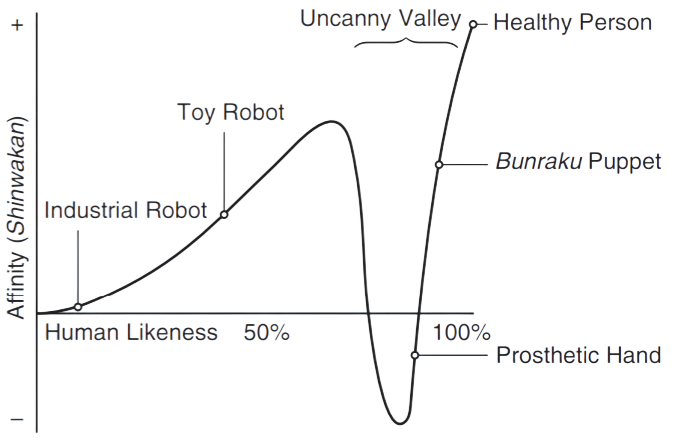
\includegraphics[width=0.5\textwidth]{graphics/uv_appearance.png}
    \caption{The uncanny valley in terms of appearance.}
    \label{fig:uv_appearance}
\end{wrapfigure}
The graph illustrates how the human-likeness at first grows linearly with regards to affinity, but at a very high but not perfect human resemblance, the affinity falls rapidly.\\ 
Overcoming the uncanny valley is, however, possible according to Masahiro Mori's hypothesis, which can be noticed by the Bunraku Puppet entry in the graph. A Bunraku is a traditional Japanese form of musical puppet theatre, and even though it might not be more human-like than a prosthetic, on close inspection, its total appearance and movement from a distance are remarkably human-like. Masahiro Mori proposed that although they are very human-like, they are not perceived as repulsive by the audience.

\section{The Effect of Movement}
Masahiro Mori's original hypothesis \cite{original_masahiro} also factored in the effect of movement on the uncanny valley. He proposed that movement profoundly impacts the uncanny valley by amplifying the peaks and valleys seen in figure \ref{fig:uv_appearance}. This phenomenon can again be better illustrated with the example of the industrial robot and the prosthetic hand. When the industrial robot is programmed to move like a human, it feels more human-like, and we feel a higher affinity towards the robot. On the contrary, when the prosthetic hand, which already creates a robust uncanny valley effect with its appearance, starts to move, the feeling of eeriness intensifies.
Figure \ref{fig:uv_movement} illustrates how adding movement steepens the slopes of the uncanny valley.
\begin{wrapfigure}{r}{0.5\textwidth} %this figure will be at the right
    \centering
    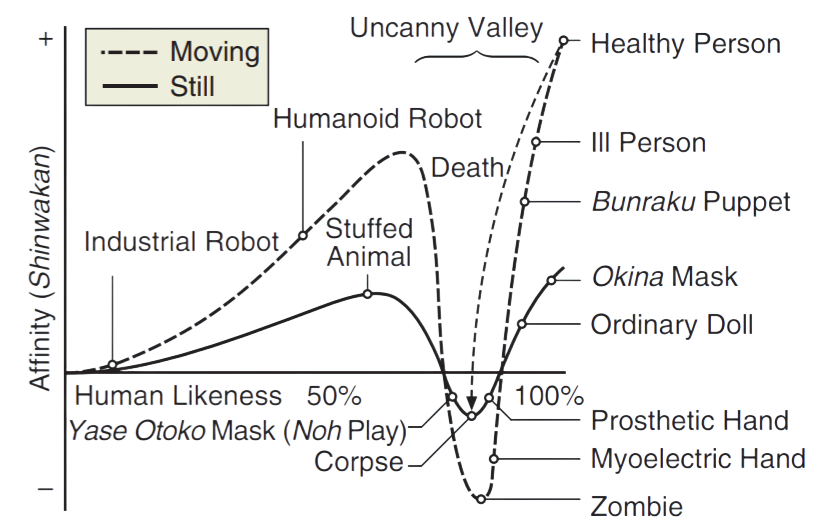
\includegraphics[width=0.5\textwidth]{graphics/uv_movement.png}
    \caption{The effect of movement on the uncanny valley.}
    \label{fig:uv_movement}
\end{wrapfigure}
Since even the movement of a single body part can have a negative effect, the unnatural movement of an entire robot can have a strong adverse effect on the affinity towards a robot. Furthermore, it is elementary for a human to recognise the slightest variations in movements which do not exactly match the human version of this movement. This can very quickly lead to an entity that has come close to a human appearance falling deep into the uncanny valley. In summary, movement can amplify the slopes of the uncanny valley proposed by Masahiro Mori.


\chapter{Variations of the Uncanny Curve}
In Masahiro Mori’s original hypothesis \cite{original_masahiro}, one can see that if an entity's appearance and movements become indistinguishable from humans, it is possible for the entity to escape the uncanny valley. Moreover, it is even possible that the affinity for an entity, which has overcome the uncanny valley, exceeds the affinity of entities which have not yet fallen into the uncanny valley. If this hypothesis holds, it would have major implications for robotics and other scientific fields as they must strive to design entities whose looks and movements are as similar as possible to that of a human being.\\
On the contrary, it may be possible that the uncanny valley  is not as clearly defined as Masahiro Mori suggests and that it could resemble an uncanny cliff or even an uncanny wall in which the affinity towards entities with perfect or near-perfect human likeness is, in general, lower than that of entities that did not fall into the uncanny valley. In these hypotheses, it may not be advantageous to strive for perfect human likeness.

\section{A Hazy Uncanny Valley}
Masahiro Mori has proposed the uncanny valley as a well-defined graph with a clearly visible dip in affinity as human likeness increases. Furthermore, movement merely steepens the slopes of the uncanny valley in his proposal.
In one of his studies, MacDorman \cite{uncanny_ambiguous} investigated whether the uncanny valley is as clearly defined as Masahiro Mori suggests. To further observe whether human likeness is the main triggering factor, he focused on using androids and robots as stimuli, performing various activities in different environments. For his study, he recruited 56 Indonesian participants, 43 male and 13 female, of whom 13 were 17 to 20 years old, 36 were 21 to 25, 4 were 26 to 30, and 3 were 31 to 35. Having been recruited in an internet cafe and mainly being university students, young professionals, and government workers, the participants had extensive technical experience.\newpage
\begin{wrapfigure}[25]{r}{0.5\textwidth} %this figure will be at the right
    \centering
    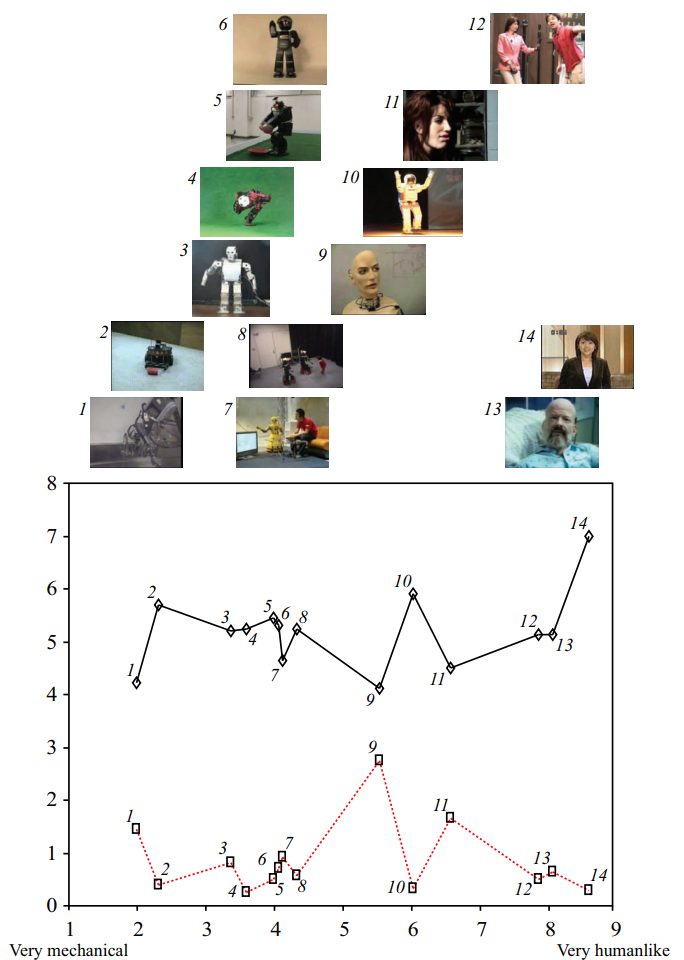
\includegraphics[width=0.5\textwidth]{graphics/hazy_uncanny.png}
    \caption{Result graph of the ratings for the 14 videos.}
    \label{fig:hazyUncanny}
\end{wrapfigure}
The study procedure consisted of a questionnaire in which the participants had to rate 14 video clips, which were 30 to 60 seconds in length, on a nine-point mechanical versus human-like scale, a nine-point strange versus familiar scale, and a
ten-point eeriness scale. The main focus was placed on the selected videos, which consisted of a mobile robot (Pioneer II), a manipulator arm, seven humanoid robots (Rovovie-M3, HR-2, VisiON Nexta, Chronio, Robovie, Wakamaru, Asimo), two android heads (K-bot, Eva), two androids (Philip K. Dick, Repliee Q1Expo), and one human being. The entities depicted in the videos performed different actions in different contexts, sometimes also with speech accompaniment.\\
Figure \ref{fig:hazyUncanny} shows the videos used together with the evaluations of the questionnaire. The solid line plots the relationship between perceived human likeness and perceived familiarity. The dashed line plots the relationship between
perceived human likeness and eeriness. The results of his study show that there is not one particular, uncanny valley for a particular range of human likeness. Therefore, the study  concludes that human likeness is only one of many factors influencing the extent of the uncanny valley effect.\\
From this study, one can conclude that in the real world scenarios with many different influences and situations in which one might encounter the uncanny valley,  it may not only be triggered by the appearance of an entity alone but by many different influences in the respective situation. This creates a much more difficult picture of the uncanny valley than Masahiro Mori suggested. However, the question of whether it is possible to overcome the uncanny valley remains open in this study.

\section{An Uncanny Cliff}
A study by Bartneck et al. \cite{uncanny_cliff} tried to plot the uncanny valley, emphasising the last ascending section of the curve. Furthermore, the referred study also dealt with the question of whether highly human-like androids are perceived as more likeable when they are being framed as robots.\\
In this study, a framing and an anthropomorphism experiment were conducted. Framing contained three conditions: human, robot and none. Anthropomorphism consisted of four conditions real human, manipulated human, computer graphic and android. Additionally, only in the robot framing condition, two additional anthropomorphisms were present: humanoid and pet robot. For the experiment, only pictures of entities that either exist or are highly similar to existing entities were chosen. 
With a questionnaire, the human likeness and the likeability of the stimuli were measured.
To ensure the framing conditions of this study, three different questionnaires with different framings of the pictures were created. The pictures were either framed as human, robot or only as a face for a neutral comparison in each different framing. For each anthropomorphism category, three different pictures were shown to the participants. 
58 people participated in the study aged between 18 and 41 years. 28 of which were female, and 30 were male.
Each of the 18 chosen stimuli was presented to the participants twice. Once with a question about the liking towards the entity, which could be rated on a scale from one to seven and once with 7-point semantic differential scales consisting of the values fake/natural, machinelike/human-like, unconscious/conscious, artificial/lifelike, nice/awful, friendly/unfriendly, kind/unkind, and pleasant/unpleasant. This resulted in 36 questions that the participants had to answer on a computer in a randomised order.\\
This study concluded that the framing of the entities had no significant influence on the measurements. The pictures were evaluated independently from whether they were labelled as human, robot or face, and the labelling did not impact the likeability or human likeness in a negative or positive way.
 However, the questionnaire results showed that anthropomorphism had a significant influence on human likeness and likeability. The participants most liked the pictures of toy robots and humanoids. Even though a slight upwards trend in likability towards highly human-like entities was noted, not even the pictures of humans reached the affection level of the pictures of toy robots. Based on these results, the study speculates that even the most human-like androids are not liked as much as toy robots or humanoids. Therefore the study suggests a revised graph of Mori's original graph where there may be small valleys, but the main feature is a cliff which is depicted in figure \ref{fig:uncannyCliff}.
\begin{wrapfigure}[13]{r}{0.5\textwidth} %this figure will be at the right
    \centering
    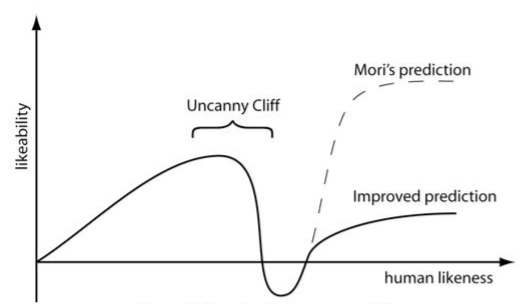
\includegraphics[width=0.5\textwidth]{graphics/uncanny_cliff.png}
    \caption{Hypothesised uncanny cliff.}
    \label{fig:uncannyCliff}
\end{wrapfigure}
In summary, figure \ref{fig:uncannyCliff} would, therefore, not describe an uncanny valley but an uncanny cliff.
The results of this study would imply that it is unwise to attempt to build highly human-like entities since a machinelike robot would be liked more. However, the study mentions that to test the hypothesis further, more studies need to be conducted with participants from different cultures, as the group of participants in the presented study consisted only of Japanese people, who are stereotypically thought of as being more avid robot-aficionados than other cultures.

\section{An Uncanny Wall}
Both in robotics and the creation of virtual characters for films and other media, ever-improving technology is allowing progress to be made towards increasing realism. Based on these improvements, Angela Tinwell and Mark Grimshaw \cite{uncanny_wall} designed a study to examine and plot the curve of the uncanny valley by using videos of virtual characters.\\
For the study, Tinwell et al. chose 100 participants, 92 of them were males and eight females, mainly university students from the creative technology field and professionals working within this academic sector and the video game industry. The selected focus group for the study consisted exclusively of people with much knowledge about informatics and game design and art and, therefore, a lot of exposure and comprehension of the uncanny valley. Furthermore, significantly more men were selected for the study and no information was given about their age.\\%TODO   
\begin{wrapfigure}[16]{r}{0.6\textwidth} %this figure will be at the right
    \centering
    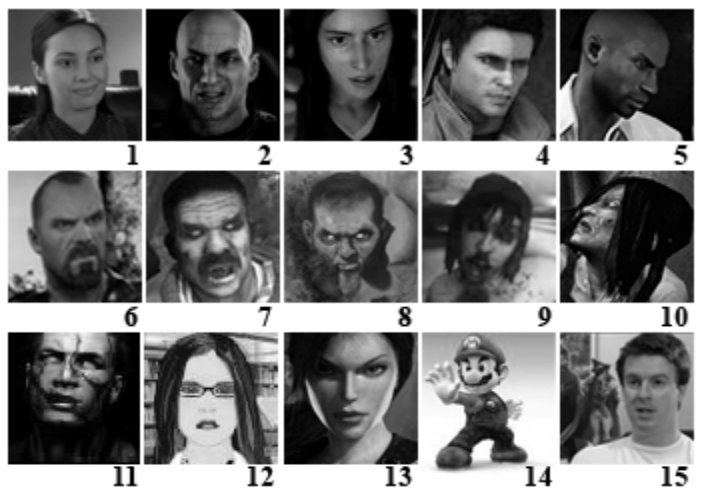
\includegraphics[width=0.6\textwidth]{graphics/uncanny_wall.png}
    \caption{The 15 characters chosen for the study.}
    \label{fig:uncannyWall}
\end{wrapfigure}
The method of the study consisted of a web-based questionnaire in which the participants had to rate 14 video clips of a selection of virtual characters and one video clip of a real human, which were placed in different settings and engaged in different activities, on a nine-point scale how human-like they perceived the characters and how strange or familiar they perceived the character. The video clips were made up of six photorealistic characters, five zombie characters, a photorealistic human-like zombie, three stylised human-like characters and one real human, as seen in figure \ref{fig:uncannyWall}\\
The study results show that the real person was found to be the most familiar and the most human-like by the participants. The six photorealistic characters were found to be very familiar and very human-like, but they could not achieve the ratings of the real person. All zombie-like characters reached shallow familiarity and low human likeness. 
The three stylised human-like characters had received very different ratings. For example, Mario from Mario and Sonic at the Olympic Games was rated as very familiar but not very human-like, and Lara Croft from Lara Croft Tomb Raider: The Action Adventure was rated as very familiar but only in the higher midfield of human likeness. 
\newpage
\begin{wrapfigure}[17]{r}{0.5\textwidth} %this figure will be at the right
    \centering
    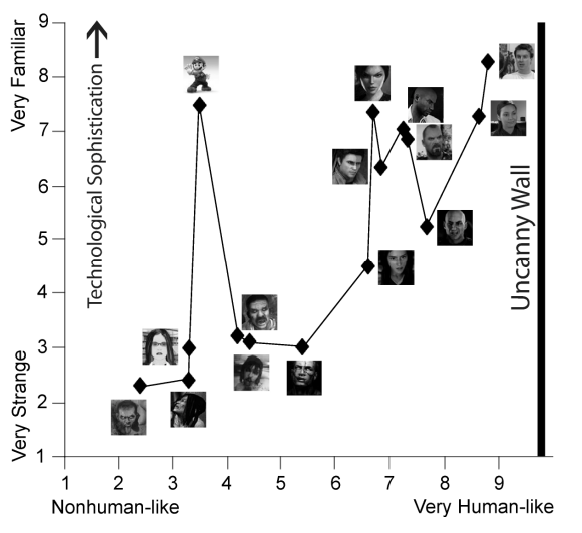
\includegraphics[width=0.5\textwidth]{graphics/uncanny_wall_graph.png}
    \caption{Hypothesized uncanny wall.}
    \label{fig:uncannyWallGraph}
\end{wrapfigure}
As seen from the constructed graph \ref{fig:uncannyWallGraph}, no single valley is found.
Therefore, it can be assumed that the uncanny valley lacks the clarity proposed by Masahiro Mori and paints a more complex picture with multiple influences affecting the familiarity with human-like entities felt by participants.  The fact that no virtual character could outperform a real person, even though all participants were previously exposed to the effects of the uncanny valley in their everyday lives, suggests that an uncanny wall can better define the uncanny valley. Therefore it may be impossible to traverse the uncanny valley defined by Masahiro Mori. Furthermore, the study assumes that with the factor of time, audiences do not get used to the uncanny valley effect, but that time leads to an increasing discernment on the part of viewers to more small details which do not perfectly resemble real humans. Through this sophistication of discernment, the uncanny wall rises with time.\\
This study thus paints a new picture of the uncanny valley, which is impossible to overcome, even with ever-improving technological possibilities. However, it is also worth mentioning that the study's statements should be again validated by conducting the study again with the new possibilities in the development of human-like designs which have emerged in recent times. In such a repeated study, more participants who are not all familiar with the subject matter should be chosen. Finally, when selecting the characters, care should be taken that they are not known to the participants to not influence their ratings.









%Brainstorm of possible next chapters respectively. what I want to include
%TODO collect empirical data to different studies through time for different groups of people maybe combine with capter 5
\chapter{What Causes the Uncanny Valley?}   
\label{chap:4}
Soon after Masahiro Mori hypothesized the uncanny valley, the question of what causes the uncanny valley arose. Viewed simply, there can only be two answers to this question. Either the uncanny valley has an evolutionary origin and therefore develops at a very young age, or the uncanny valley arises through external influences over one's life experiences, therefore having a societal origin. 
\section{Explanatory Hypotheses of the Uncanny Valley}
According to Strait et al. \cite{childrens_responding}, there are two primary perceptually oriented hypotheses which thus support the evolutionary origin of the uncanny valley: the category ambiguity hypothesis and the feature atypicality hypothesis.\\
The category ambiguity hypothesis \cite{childrens_responding} is based on the difficulty, for us humans, in categorising very but not completely human-like entities. This categorisation has evolved in the course of our evolution and is one of the most basic human cognitive abilities. The valley-related discomfort is thus triggered when an entity cannot be categorised easily, which is the case at category boundaries, for example, the robot-human boundary. The category ambiguity hypothesis may also suggest that the uncanny valley is unavoidable due to the automatic categorisation humans experience when looking at different entities.\\
The feature atypicality hypothesis \cite{childrens_responding} argues that the uncanny valley originates in atypical features of figures that violate the expectations of their appearance or behaviour. An example of this would be a figure with a human-like head and a mechanical body. Such a figure would thus violate our expectations of how an actor should look or behave. Therefore this theory proposes that overall consistency regarding anthropomorphic or mechanomorphic features could avoid the uncanny valley effect.\\
The category ambiguity hypothesis and the feature atypicality hypothesis both explain the emergence of the uncanny valley through evolutionary processes. Otherwise, there is the theory that the uncanny valley arises through social influences over the course of a lifetime. Social triggers here could be, for example, the fear of humans being replaced by machines, which is spread by films or similar media. According to this theory, the uncanny valley would thus only develop with exposure to specific social influences and should therefore be less or not at all present in children or people who have been avoiding these social influences. 
\section{Differentiating Between the Explanatory Hypotheses}
In order to find the origin of the uncanny valley, we must first distinguish between the major opposing theories. Is the uncanny valley caused by our perception and has, therefore, an evolutionary origin or by social influences? After a consensus has been found in existing studies, it is possible to differentiate between either the two main hypotheses in the perceptually oriented direction, the category ambiguity hypothesis and the feature atypicality hypothesis, or between different influences that could cause the uncanny valley through social effects. The following discusses studies that have conducted experiments, testing whether the uncanny valley is already present in infants and children.
\subsection{Development of the Uncanny Valley in Infants}
A study by Lewkowicz et al. \cite{uncanny_infants} investigated the visual preferences of 6-, 8-, 10- and 12-month-old infants towards human faces, realistic avatar faces, and uncanny avatar faces to understand the synergy of evolutionary and developmental influences on the maturing of the uncanny valley effect. For their experiment, they chose 96 infants of mostly Caucasian phenotype and conducted three experiments in which they presented all possible pairs of three types of faces containing two human faces, two uncanny avatar faces and two realistic avatar faces, as seen in figure \ref{fig:uncannyInfants}, to the infants. 
\begin{wrapfigure}[13]{r}{0.6\textwidth} %this figure will be at the right
    \centering
    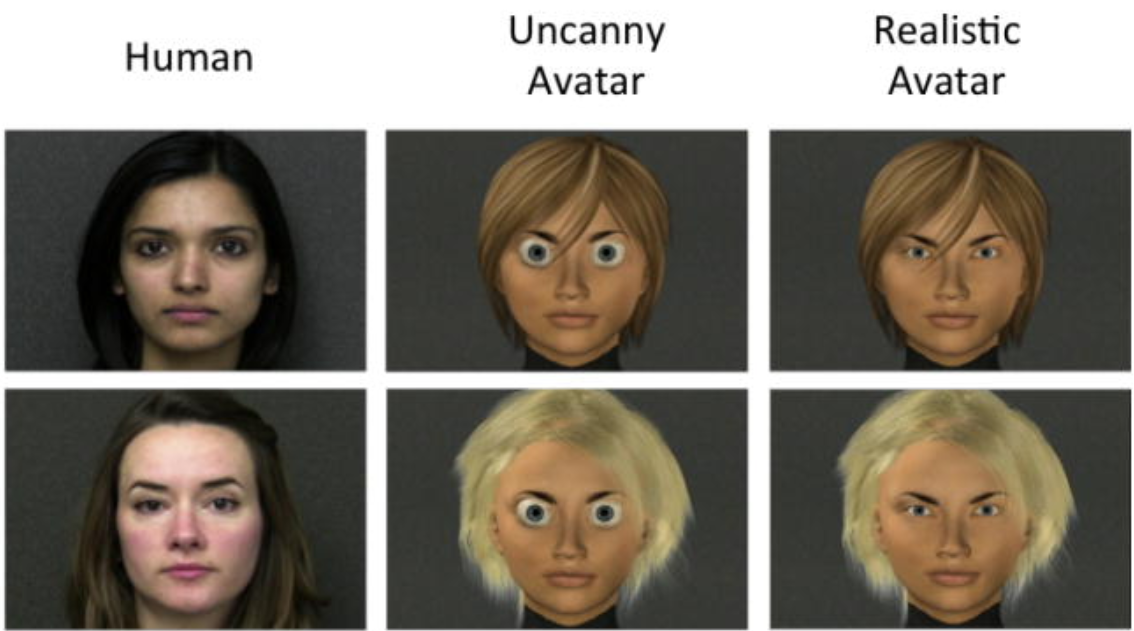
\includegraphics[width=0.6\textwidth]{graphics/uncanny_infants.png}
    \caption{Images of the three different types of faces.}
    \label{fig:uncannyInfants}
\end{wrapfigure}
In the first experiment, the uncanny avatar faces were combined with the human faces to monitor the infants' time to look at the different faces. The uncanny avatar faces were paired with the realistic avatar faces for the second experiment. The main difference between the realistic and uncanny faces were the unrealistically large eyes of the uncanny faces. Therefore, this experiment tested mainly whether infants are sensitive to large eyes by monitoring the time the infants looked at the different faces. In the third experiment, the realistic avatar faces were combined with the human faces to test if the response of the first experiment would be based on the eye size or if the infants were more sensitive to how closely the faces resembled a human prototype.\\
This study provides a fascinating new insight into the uncanny valley effect. The first experiment showed a dramatic shift in infant response to the uncanny avatar faces and human faces depending on their age. The 6-month-old infants preferred the uncanny avatar face instead of the human face, while the 12-month-old infants preferred the human face instead of the uncanny avatar face. Therefore, the uncanny valley effect is not yet present in the first six months of life, but it develops during the second half of the first year.\\
The second experiment confirmed that the infants are susceptible to eye size differences and that they preferred the faces with normal-sized eyes.\\
The results of the third experiment verified that the infants mainly paid attention to the eyes and did not recognise the synthetic nature of the realistic character. This further proved the study's main finding that infants looked less at the uncanny avatar because of the unusually large eyes.\\
In summary, this study suggests an interplay between the early influences on infant development and evolutionary mechanisms as the cause of the uncanny valley. Once infants have learned the prototype, they likely have sufficient perceptual experience to recognise irregularities in imperfect human-like entities, triggering the uncanny valley. It is also clear from previous studies that perceptual abilities are relatively crude at the start of life but improve rapidly during the first year \cite{Lewkowicz2009_perceptual_abilities,Pascalis2009_perceptual_abilities}. Specific developmental experiences of faces and emotions let their observers quickly learn to recognise abnormalities and aesthetic values of a face. As a result, faces that are abnormal/not human-like have a repulsive effect which causes an uncanny valley effect.\\\\
Matsuda et al. \cite{uncanny_infant_discrimination} conducted a similar study testing infants' discrimination against humanoid robots. In the study, an experiment showing three different types of agents to 42 infants aged between 6 to 14 months was conducted. The chosen visual stimuli consisted of three different black and white video clips, which pictured a human, an android and a mechanical robot performing a grasping action with their right hand, as shown in figure \ref{fig:uncannyInfantsDiscrimination}. The infants were each shown two different videos of the agents, which were played side by side. 
\newpage
The videos were paired into human and android, human and robot, and android and robot combinations. Each pair was shown to the infants four times for 10.5 seconds. During the experiment, the children were sitting on their parents' laps, who were instructed not to react either to the shown agents or to the infants. In order to analyse how the infants react to the different agents, their eye movements were monitored in real-time.
\begin{wrapfigure}{r}{0.6\textwidth} %this figure will be at the right
    \centering
    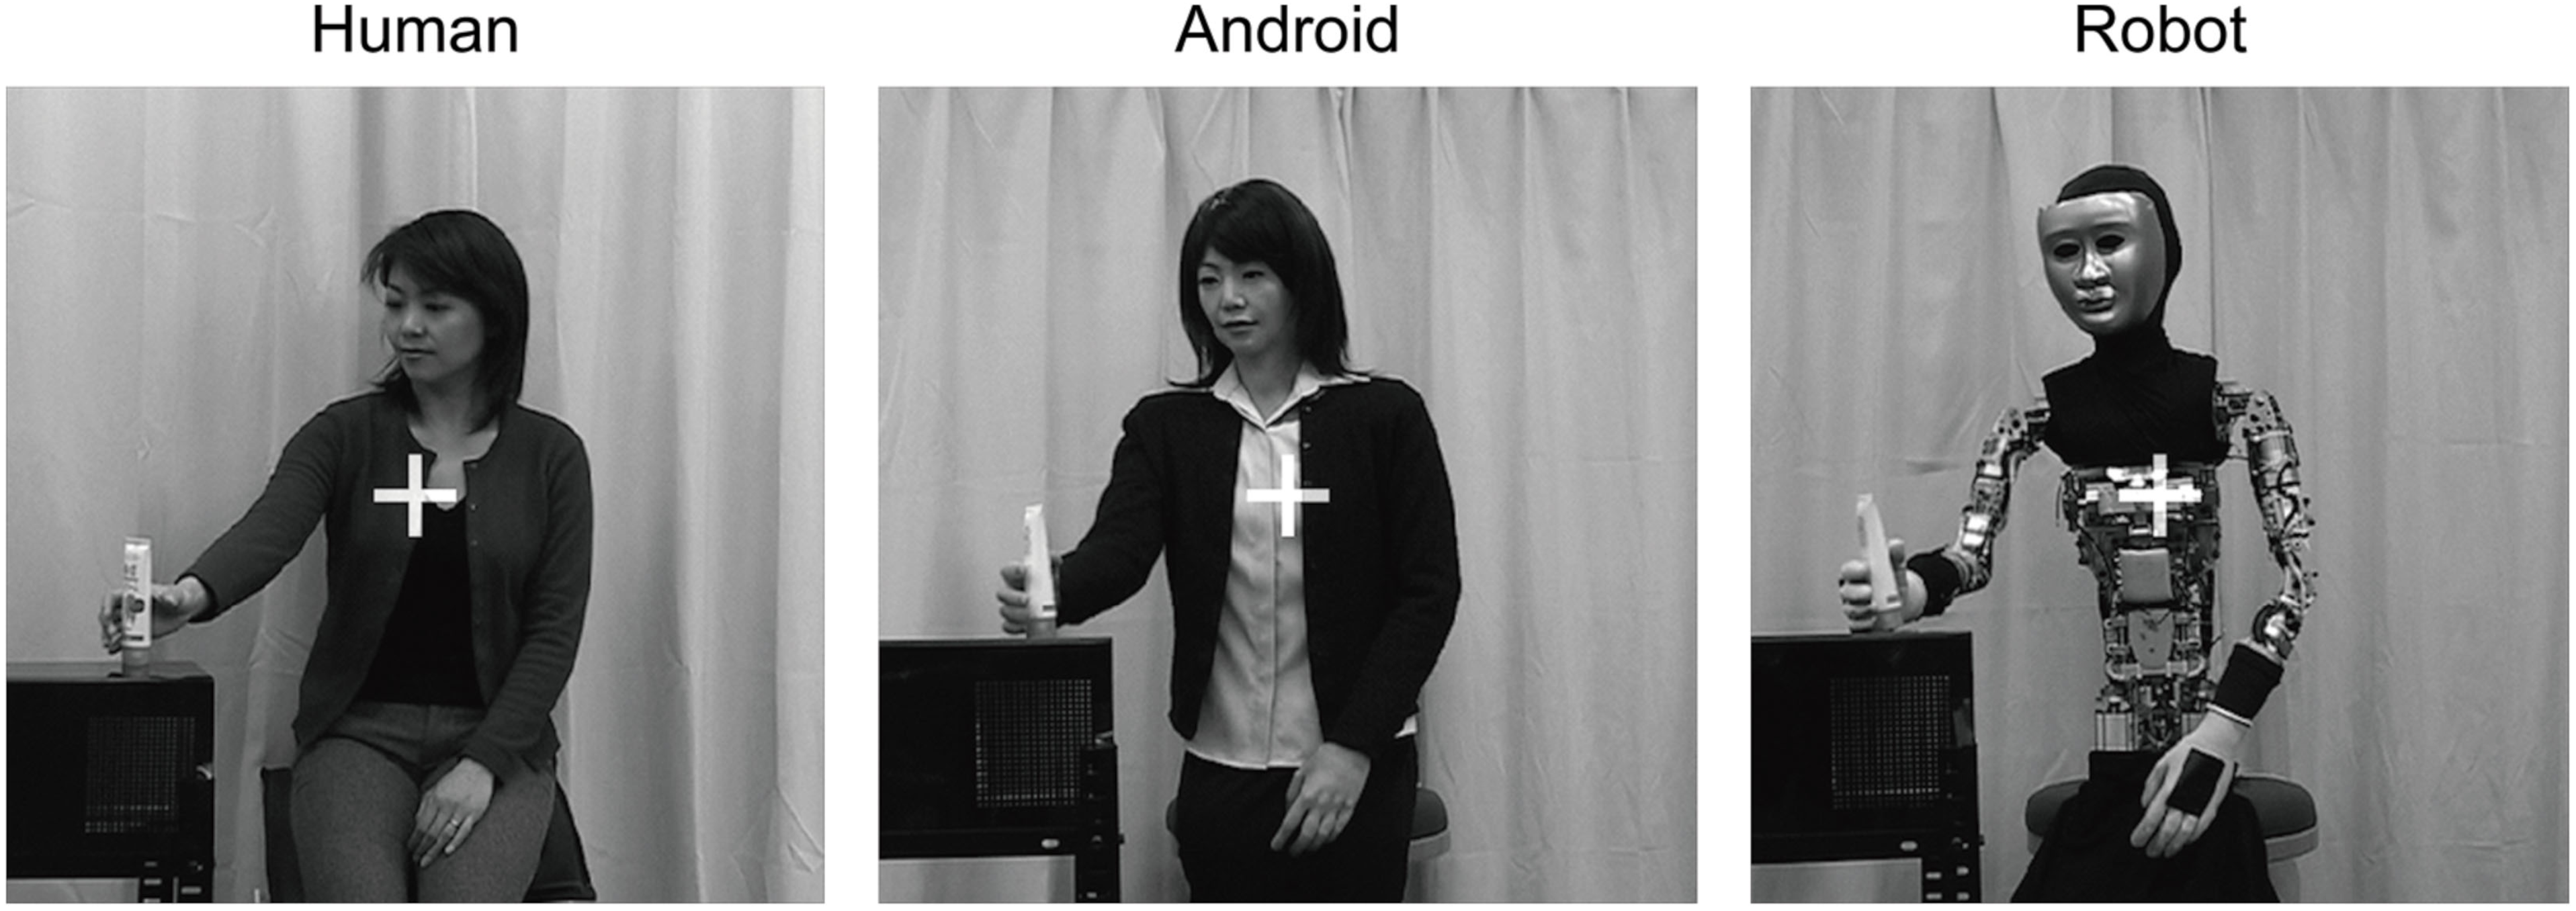
\includegraphics[width=0.6\textwidth]{graphics/uncanny_infants_discrimination.png}
    \caption{Images of the three different types of agents used.}
    \label{fig:uncannyInfantsDiscrimination}
\end{wrapfigure}
The experiment results show that the infants spent the longest time viewing the robot. In contrast to studies conducted with adults, there was no difference in the viewing time between the human and android agents. So this study suggests that infants up to 14 months of age do not yet have the perceptual abilities to distinguish between the human and android looking agents. However, it seems that they are already able to distinguish humans from robots. Since infants tend to observe novel objects, this could be a possible reason why they looked at the robots longer. In summary, this study did not find discrimination against androids in infants. From the study results, it can be suggested that the infants' perceptual abilities were not yet well enough to recognise the subtle differences between the human and android agents. As a result, the infants had not yet developed an uncanny valley effect.\\\\
When comparing the two studies, one can see certain similarities but also disagreements. The study by Lewkowicz et al. \cite{uncanny_infants} proposes that infants would learn the necessary perceptual abilities gradually in the second half of their first year of life to differentiate between human agents and human-like android agents. In contrast, the study by Matsuda et al. \cite{uncanny_infant_discrimination} could not find evidence that infants aged 14 months could differentiate sufficiently between the android agents and the human agents. However, they could already distinguish between humans and robots. By looking at the characters used by Lewkowicz et al. and Matsuda et al., one can see that the differences in the study by Matsuda et al. between the human and the uncanny agent are very subtle. On the contrary, the uncanny avatar from the study by Lewkowicz et al. can easily be distinguished from the human face. This may be the reason for the lack of response from the infants to the android agents in the study by Matsuda et al.. Concluding, it seems that the development of the uncanny valley goes hand in hand with the development of perceptual abilities in infants. This development seems to occur between the 6 and 14 months of an infant’s life, but the full development of these skills may depend on the individual’s developmental rate. This may explain the different results of the two studies. 
\newpage

\subsection{Observing the Uncanny Valley in Children}
To investigate the existence of the uncanny valley effect in children, Strait et al. \cite{childrens_responding} researched children's reactions, ranging from 5 to 10 years in age, to figures with different human-likeness and ordinary people. For the study, 80 children were recruited from a science museum. The children were shown a total of 24 different characters, which were divided into four categories of appearance: robot-like, humanoids with an atypic appearance, humanoids with an ambiguous appearance, and humans. The stimuli used for the experiment are depicted in figure \ref{fig:childrensRespondingAvatars}.
\begin{wrapfigure}{r}{0.5\textwidth} %this figure will be at the right
    \centering
    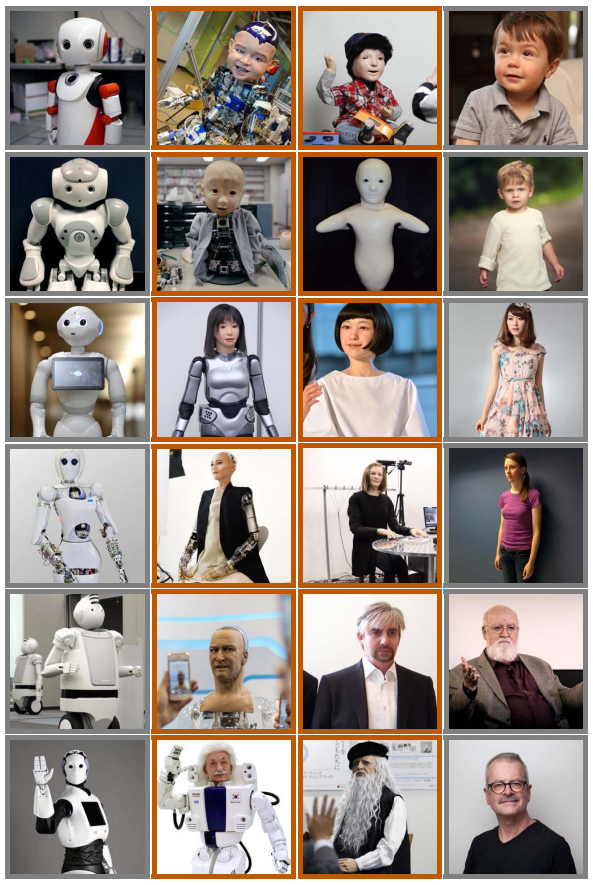
\includegraphics[width=0.5\textwidth]{graphics/childrens_responding_avatars.png}
    \caption{Images of the different figures used.}
    \label{fig:childrensRespondingAvatars}
\end{wrapfigure}
The six characters of the last column depict the humans; the remaining 18 are of little resemblance to humans, i.e. very robot-like to very human-like. To distinguish between the category ambiguity hypothesis and the feature atypicality hypothesis, the second column depicts humanoids with atypical features, such as a robot with a human head. The third column depicts humanoids with an ambiguous ontology.\\
The experiment consisted of two tasks.
First, the children had to complete an observation task in which they looked at the pictures for 12 seconds until the next picture appeared. During the 12 second observation time, the children could terminate at any time, which would take them to the following picture. This task was followed by a preference assessment in which the children were presented with four pictures from every category, mechanical, atypical, ambiguous  and human. The children were asked to indicate which of the four figures they liked most and which of the images they preferred the least.\\
The results of this study were analysed based on four indices, the dislike frequency and like frequency derived from the second task and the termination frequency and viewing duration from the first task.
The data from these indices showed that the children preferred the mechanical agents the most, followed by the real humans. 
However, they were averse to the very but not quite human-like entities, making their behaviour resemble the uncanny valley effect. Furthermore, from the dislike/like frequency data, a greater aversion towards the atypical characters than the ones with an ambiguous ontology could be identified. This study, therefore, showed that the aversion is driven more by atypicality than by ambiguity which thus supports the theory of the feature atypicality hypothesis. As there were no discernible differences in behaviour between the different age groups, the study assumed that the uncanny valley is of evolutionary origin and not triggered by social influences.\\

\section{External Influences on the Uncanny Valley}
From the discussed studies, it can be concluded that the uncanny valley has its origin in evolutionary mechanisms and evolves with the perceptual abilities in early childhood development. Based on research with children, Strait et al. \cite{childrens_responding} further inferred that there is a greater aversion towards atypical entities than entities with an ambiguous ontology, thus supporting the category ambiguity hypothesis. However, the study does not rule out the possibility that social influences may negatively or positively influence the uncanny valley. From the studies discussed it can be concluded that an effect of social influences on the perception of the uncanny valley could have a significant role in the design and handling of social robots and similar human-like entities. For example, a positive influence would mean that the more, people are exposed to the uncanny valley, the less they are influenced by it. However, the opposite effect, a strengthening of the uncanny valley through social influences, is also possible.\\
Alvarez Perez et al. \cite{prior_exposure_robots} investigated in their study if the uncanny valley also manifests with exposure to robots. For his study, two groups of participants were recruited, one with no previous exposure to robots and the other who had previously interacted with Nao, a humanoid robot from the French robot manufacturer Softbank Robotics. The procedure and stimuli were similar to the study by Strait et al.. The study concluded that the human-like actors triggered an uncanny valley in the participants. Furthermore, no attenuation of the uncanny valley could be shown with participants who had already been exposed to human-like robots. Both groups of participants experienced the uncanny valley effect in the same way. So this study could not find any improvement or worsen of uncanny valley by previous exposure to robots. At this point, however, a need for future research can be identified. There is a lack of studies on the influence of external factors such as media, films or cultural and social differences on the uncanny valley.

\chapter{A Review of Existing Research}
Nowadays, the uncanny valley has a broad influence on many disciplines with different research approaches. The previous chapters also show that the uncanny valley does not have a precise definition. A consequence of these factors is that studies tailor the stimuli, terms, assessment methods, and study participants to their exact research case, leading to inconsistent results in the conducted studies.
This chapter aims to provide an overview of these differences and describes the different stimuli, terms, evaluation methods and study participants of the studies mentioned in this paper, in addition to other relevant studies, following the structure of the quantitative analysis conducted by Jie Zhang et al. \cite{quant_review}.

 \section{Deficits of existing research}
 From the comparison of the studies described in this paper as well as other selected studies and the additional input of the literature review conducted by Jie Zhang et al. \cite{quant_review}, inconsistent conditions in existing studies could be found, which can lead to uncertain results. In the following, these conditions are described, and possible recommendations for their improvement are suggested. 

\subsection{Deviating and Inaccurate Terms}
Finding correct terms to describe feelings of social closeness, familiarity, attachment and affinity, or the opposite, feelings of fear, repulsion, aversion and eeriness towards robots and human-like entities is very difficult. Different people can interpret these terms, with which they are to evaluate entities, very individually. This can lead to a distortion of the real feelings towards the entities and thus also change the whole interpretation of the uncanny valley.\\
In the first formulation of the uncanny valley hypothesis in 1970 by Masahiro Mori \cite{original_masahiro_not_translated}, he used the two terms "shinwakan" and "bukimi" to describe the feelings towards different human replicas. The word "bukimi" could be clearly translated to eeriness, however, the word “shinwakan” was proven to be complex to translate \cite{quant_review}. At first, the word “shinwakan” was translated into familiarity by Jasia Reichardt \cite{first_translation}, but later, Masahiro Mori revised the translation into affinity. Furthermore, it has also been argued by \cite{uncanny_cliff} that "likeability" would be an even more appropriate translation. Based on the dictionary definitions of these terms, they all describe slightly different aspects of perceptual familiarity and emotional valence.\\ Given these terms' complex definitions and ambiguous character, a possible solution would be self-reporting questionnaires for measuring affinity. However, this option would not be feasible for every study due to the lack of uniformity and the resulting margin for interpretation of the given answers. So an essential step for future research would be to develop a common metric for the affinity dimension. The first step in this direction would be to agree on a translation of the term "shinwakan". Furthermore, studies also need to explore how participants perceive the expressions used and draw conclusions about how they value the different entities based on the expressions. 
%Tabelle

%%%%%
\subsection{A Wide Range of Stimuli}
Like describing feelings, it is difficult to give an exact definition of a figure's degree of human likeness. As a result, the selected stimuli can vary significantly between studies, and unnecessary additional variables are often introduced. 
%Table 1 compares the different stimuli from several studies.
It can be seen that participants have to evaluate a whole range of different stimuli, including images, videos and interactions and these often have different descriptions and are often staged differently. Moreover, often only a part of the entities is depicted, such as face, head or body.
Creating standardised stimuli for studies turns out to be very difficult. Researchers should not, select their entities arbitrarily or subjectively, because no accurate conclusions about the uncanny valley could be drawn. 
One way to solve the selection problem is to morph entities. This can create a meaningful comparative series from which good conclusions of human likeness and uncanny valley can be drawn. However, this approach cannot be used for every study. As Masahiro Mori has already assumed, the uncanny valley is not limited to appearance alone, but also to movement and other external influences. In order to explore these as well, studies need to use more complex stimuli. However, this leads back to the original problem.  In order to facilitate the selection, a kind of guideline for evaluating the human likeness of different entities would be needed in order to be able to objectively select the stimuli for studies. 
%abot database bewertung erwähnen
%stimme
%Tabelle
%%%%%%

\subsection{Participants from Different Cultures and Age Groups}
When selecting participants for a study, age-related and cultural differences, as well as personal differences, must be taken into account.\\
Yun-Chen et al. \cite{age_differences} conducted a thorough study examining the uncanny valley effect throughout different age groups and concluded that the uncanny valley is perceived very differently by participants of various age groups. Younger adults
preferred non-human-like robots, while middle-aged adults showed a preference for human-like robots. Surprisingly, the study even concluded that the uncanny valley was not observed in older adults. This would mean that the uncanny valley effect weakens with advancing age and possibly disappears completely. Considering the age-related differences found in this study, future research should take age as an essential factor that profoundly affects the uncanny valley. Due to the lack of comparative studies with older people or comparisons in different age groups, research in this direction is still very limited. Therefore research in this direction is urgently needed, especially concerning social robots for older adults.\\
Furthermore, most studies do not look into the participants' cultural differences and personal experiences. Other cultures have different ways of dealing with robots. In western culture, robots are portrayed as frightening machines \cite{japan_robot_friendly}. The opposite is true in Japan \cite{japan_robot_friendly}. Here, robots are much more accepted and widespread in society due to government promotion and a generally friendlier narrative \cite{japan_robot_friendly}. The effect of cultural, social and external influences on the uncanny valley has not yet been widely researched, and it is not unthinkable that they have a significant impact on the strength of the manifestation of the uncanny valley effect. The same applies to the personal exposure and experience to the uncanny valley. It could be assumed, for example, that a person who interacts with social robots in their everyday life does not feel the uncanny valley as strongly as a person who has never had contact with a robot.\\
Therefore, studies should pay attention to their participants' cultural, social, and personal environments. More research is needed in this direction to define the effects of these influences on the uncanny valley.




%Die Assessment Methoden?
%Aus den Vergleichen soll dann ein bestimmter Schluss gezogen werden (etwa, dass die Forschung sehr uneinheitlich ist und wahrscheinlich Bedarf an gewissen genormten Studien besteht)



\chapter{Exploring the Uncanny Valley in Human-Like Robot Recruiters}
\label{chap:6}
Human resource operations are progressively becoming more digital. Many procedures are already automated, and the use of artificial intelligence is also becoming increasingly common. Especially in the recruitment process, a new approach called robot recruiting is being applied. Robot recruitment describes a semi-automatic process in which algorithms and artificial intelligence take over parts of the typical recruiting process, such as assessing and selecting applicants \cite{vera}. By analysing vast amounts of data, these algorithms are trained to assist companies in making predictions and decisions on future employees \cite{robot_recruiting_scholar}. This assistance is hoped to shorten the time-consuming process of personnel recruitment and employ a more neutral way of evaluating the applicants \cite{robot_recruiting_scholar}.\\
Many people are already familiar with websites that provide a chat window where one can talk to supposed employees. Often these 'employees' are, in fact, algorithms with which you can communicate, and they can perform a variety of simple tasks \cite{vera}. These algorithms are among the best-known applications similar to the intention of robot recruiting. When applying this concept to the recruitment processes, an algorithm takes over the simpler communication and carries out sorting, admission and possibly an exclusion of applicants \cite{vera}. However, with the rapid development of information technology, robot recruiters can take on even more complex tasks, such as conducting a job interview \cite{vera}. For this task, however, the algorithms need a medium with which to communicate with candidates, and a human-like figure in the shape of an online character or a robot is frequently used for this purpose. One example of this is a Russian start-up which has developed a robot recruitment system called robot Vera, with which companies can conduct telephone interviews with applicants \cite{vera}. This robot recruiter talks to the applicants self-sufficiently and responds to their questions. During the telephone interview, the robot takes on a female human form \cite{vera}.
With the development of a human-like appearance of robot recruiters, the effect of the uncanny valley on them also becomes relevant. If the appearance of a robot recruiter falls into the uncanny valley, it could affect the applicant's acceptance of the recruiter during the interview. This could negatively impact the applicant's behaviour and, therefore, their performance during the application process.
With the help of an online survey based on rating potential robot recruiters with varying human-likeness, this thesis explores how applicants' feelings toward different designs of robot recruiters vary. With the survey results, the thesis then tries to determine if very but not perfectly human-like robot recruiters fall into the uncanny valley. The results are also used to make a recommendation for the aspired degree of human-likeness of such entities. 

\section{Stimuli}
For the survey, eight images \ref{fig:image-1} - \ref{fig:image-8} of possible robot recruiters with different degrees of human-likeness and a control image of a real human \ref{fig:image-9} were selected. When choosing the entities, special consideration was given to the fact that they either currently exist or may be plausible as a design for a robot recruiter. Among the images are four avatars that are currently in development or use. Figure \ref{fig:image-2} shows the existing Robot Recruiter, Tengai, a physical robot developed to assist recruiters and hiring managers. More information about the company and this robot recruiter can be found on the company's website (https://www.tengai-unbiased.com/tengai-robot/). Image \ref{fig:image-5} shows a design of the robot recruiter Vera, which is developed by a Russian start-up company \cite{vera}. Figure \ref{fig:image-3} shows an avatar of the Microsoft Mesh system, which is currently under development and aims to connect people working remotely in virtual space via Mixed Reality with the help of avatars \cite{microsoft_mesh}. Although this system was not specifically designed for robot recruiting, such a design could easily be imagined. Image \ref{fig:image-4} shows the humanoid robot Sophia, which was developed by the Hong Kong company Hanson Robotics. Sophia became internationally known due to its particularly human appearance and behaviour compared to previous robot variants. The remaining figures \ref{fig:image-1}, \ref{fig:image-6}, \ref{fig:image-7}, \ref{fig:image-8} were chosen to represent a broader range of human-likeness levels and to compare existing appearances to other possibilities. The images are ordered in ascending human-likeness, which was objectively assessed by using the Human-Likeness Predictor of the Abot Database (https://www.abotdatabase.info/) and by the addition of the study's evaluation, which is discussed in the following sections. The constant values from figure \ref{fig:image-5} to \ref{fig:image-8} can be explained by the evaluation of the Abot database, which in its current state only gives a rough assessment, and the variations in the human-likeness of the picked entities are already very modest.
\begin{table}[b!]
\centering
\resizebox{\linewidth}{!}{%
\begin{tabular}{ll|ll|ll}
\ref{fig:image-1} &Human-Likeness: 47.27 &\ref{fig:image-4} &Human-Likeness: 88.72 &\ref{fig:image-7} &Human-Likeness: 94.55 \\ \hline
\ref{fig:image-2} &Human-Likeness: 65.16 &\ref{fig:image-5} &Human-Likeness: 94.55 &\ref{fig:image-8} &Human-Likeness: 94.55 \\ \hline
\ref{fig:image-3} &Human-Likeness: 84.13 &\ref{fig:image-6} &Human-Likeness: 94.55 &\ref{fig:image-9} &Human-Likeness: 100
\end{tabular}
}
\caption{Rated human-likeness of the figures.}
\label{tab:rated-human-likeness}
\end{table}
\newpage

\begin{figure}[t!]
 \centering
 \subfloat[\cite{icup}\label{fig:image-1}]{%
      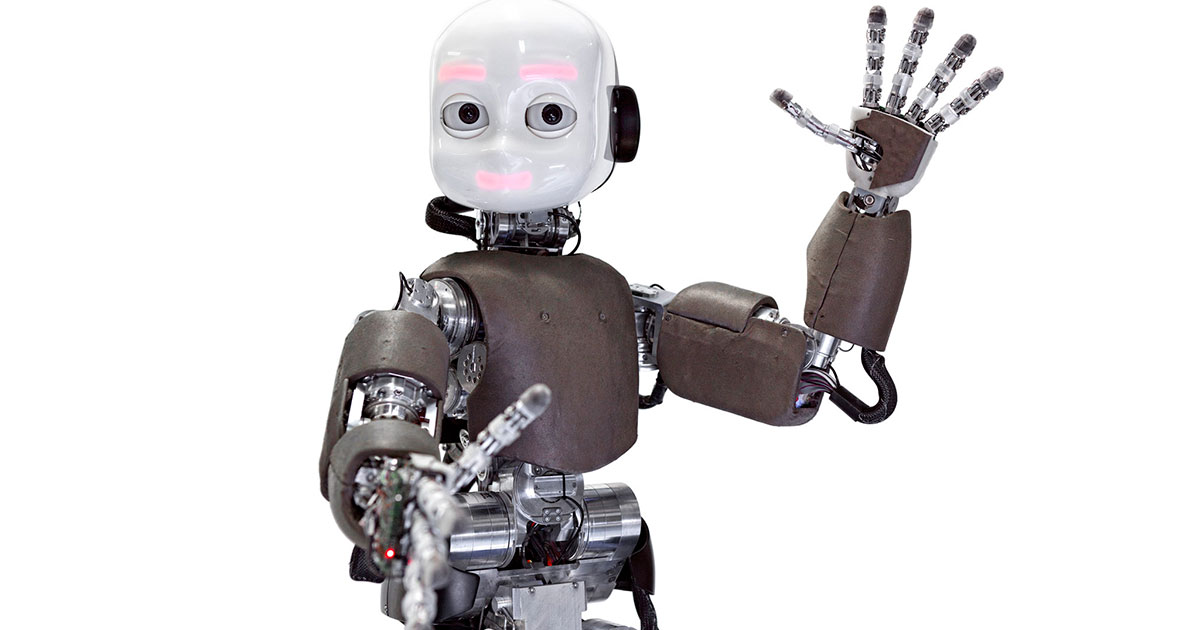
\includegraphics[width=0.26\textwidth]{graphics/study/icup.jpg}}
 \qquad
 \subfloat[\cite{tengai}\label{fig:image-2}]{%
      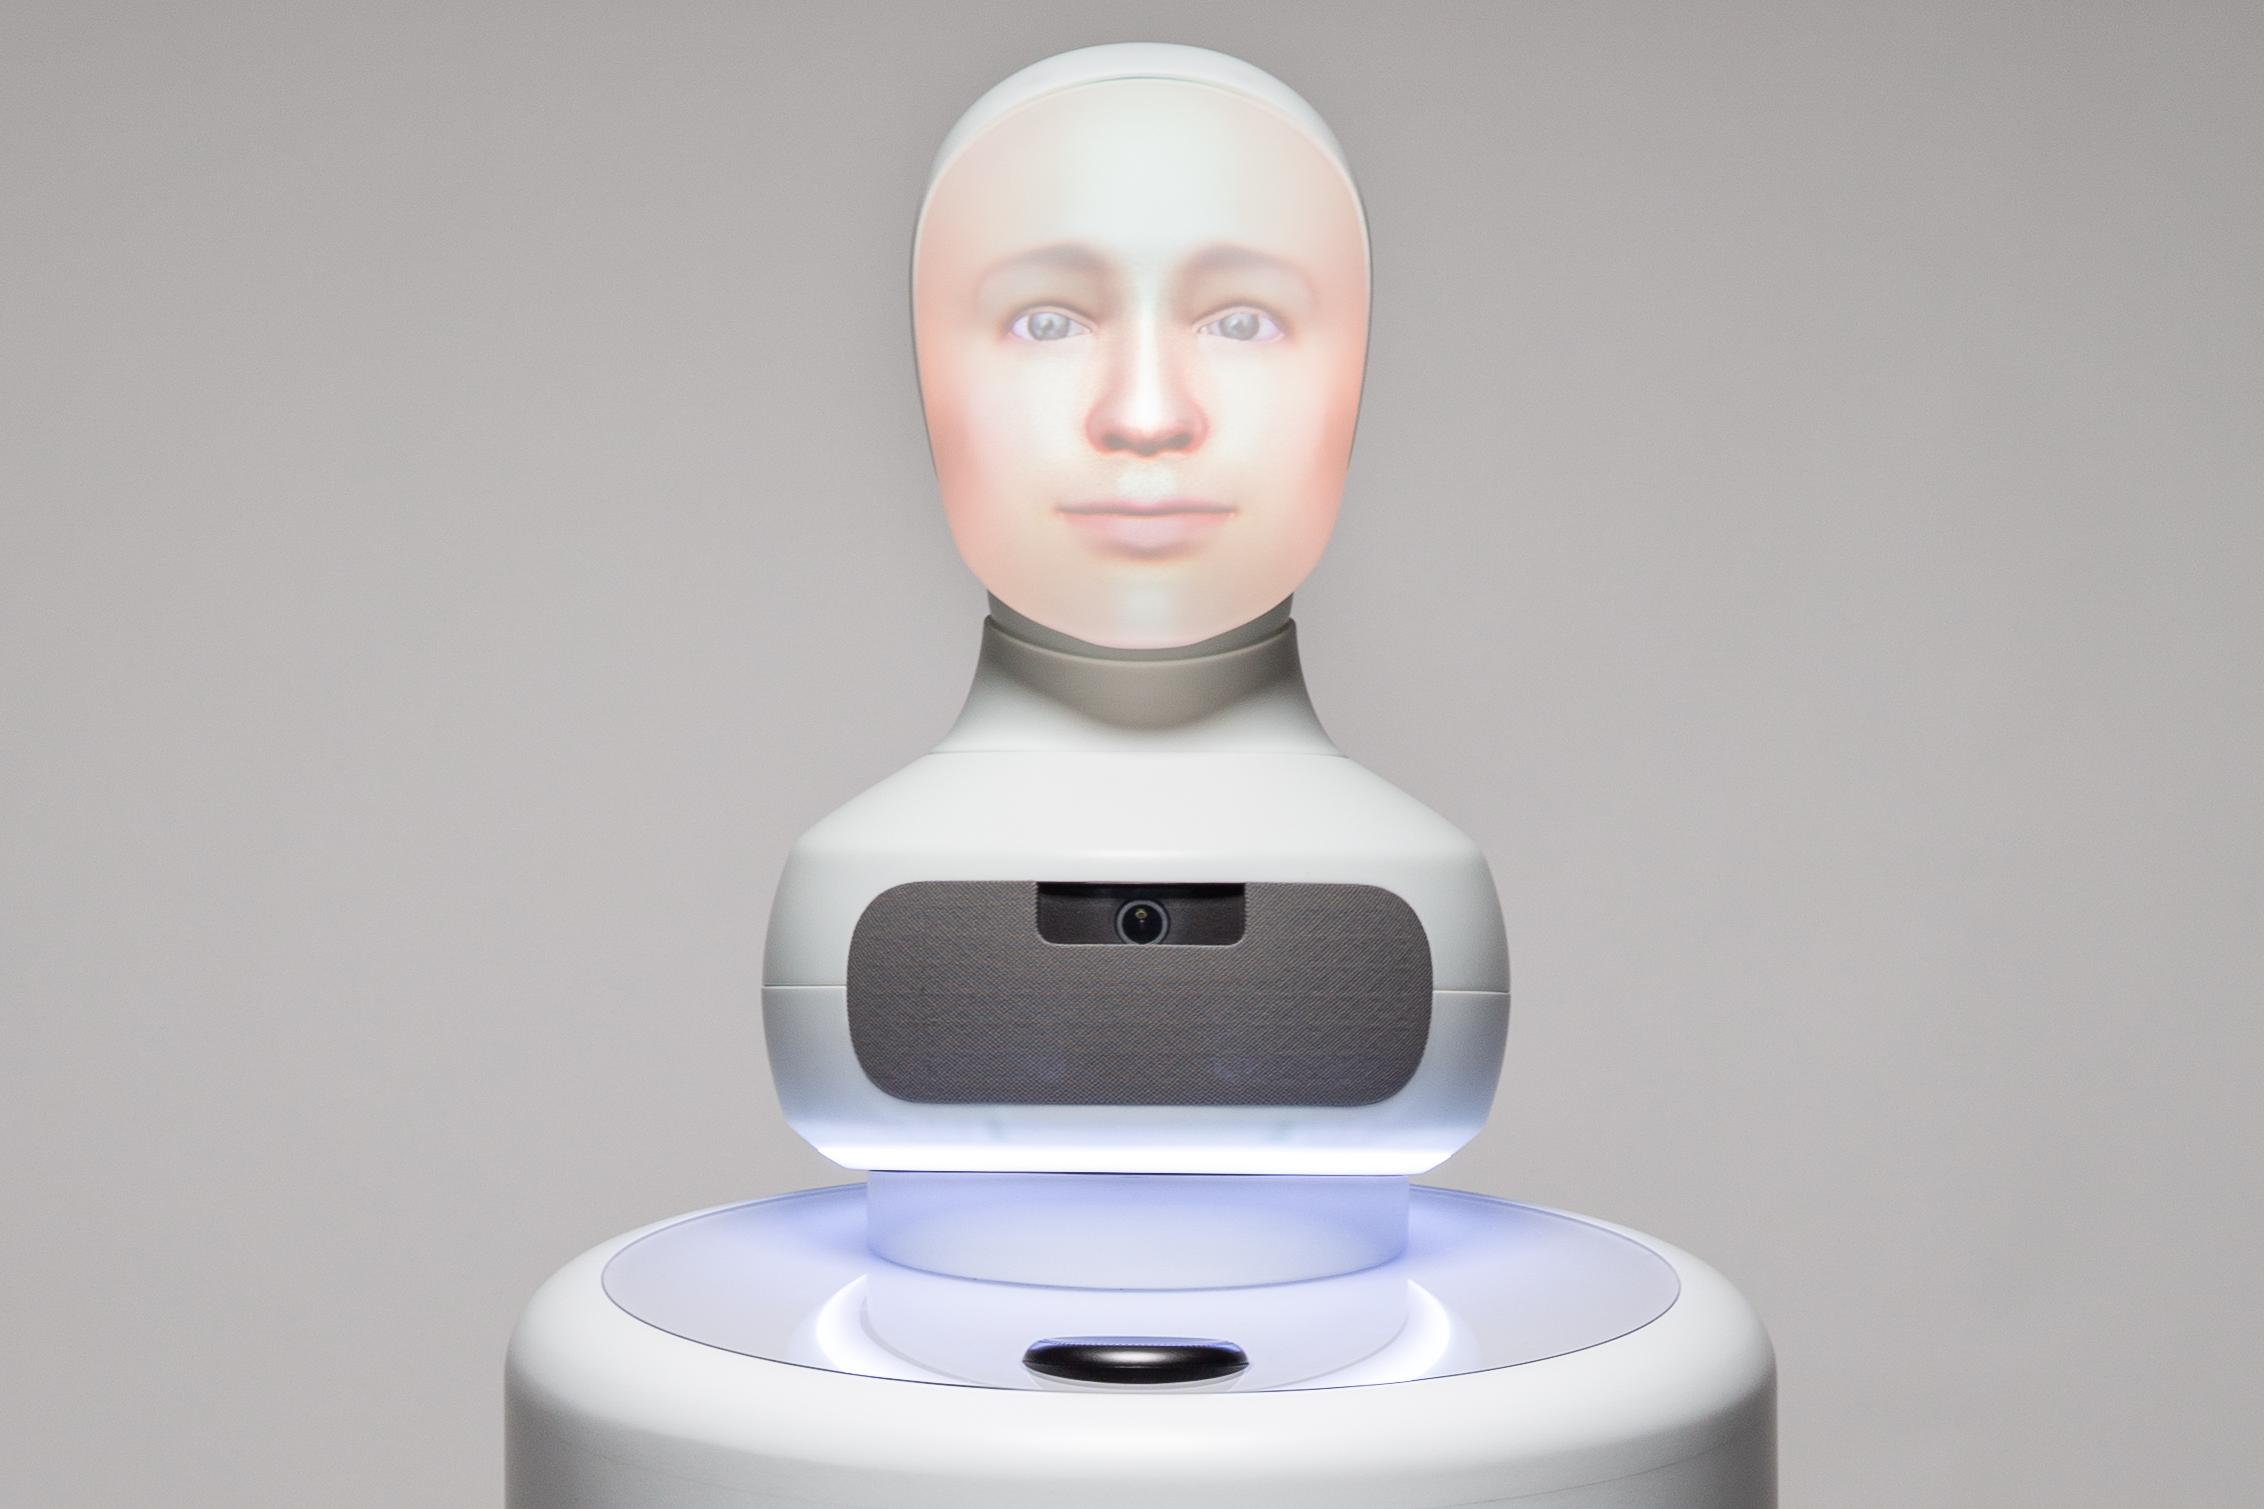
\includegraphics[width=0.26\textwidth]{graphics/study/tengai.jpg}}
 \qquad
 \subfloat[\cite{microsoft_mesh}\label{fig:image-3}]{%
      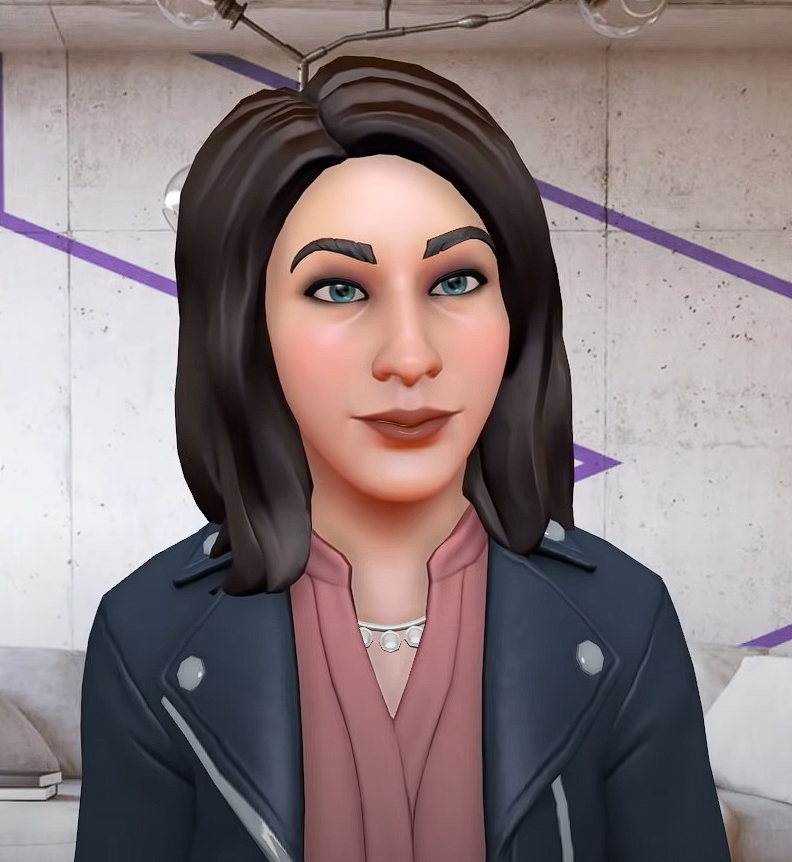
\includegraphics[width=0.26\textwidth]{graphics/study/microsoft_mesh.png}}
      
 \centering
  \subfloat[\cite{sophia}\label{fig:image-4}]{%
      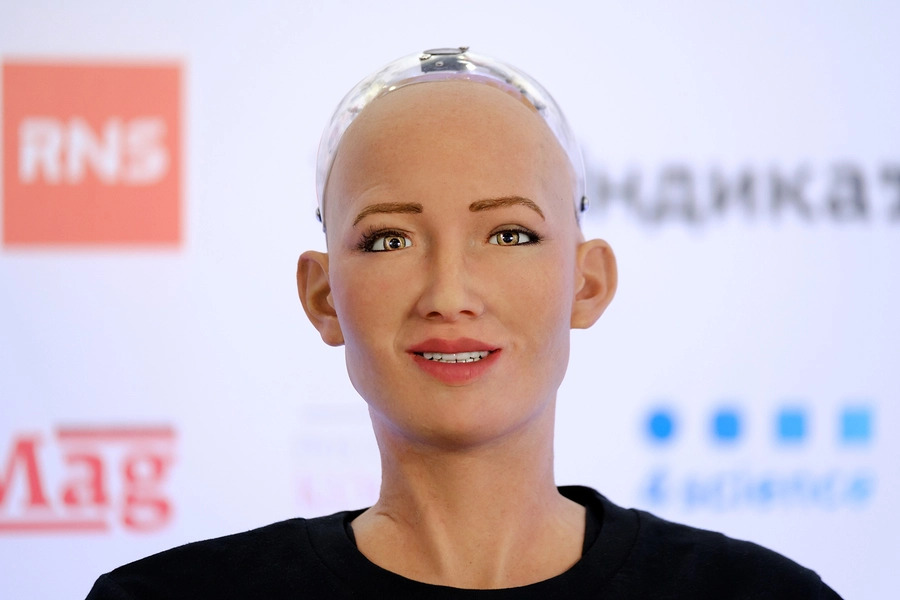
\includegraphics[width=0.26\textwidth]{graphics/study/sophia.jpg}}
 \qquad
 \subfloat[\cite{vera}\label{fig:image-5}]{%
      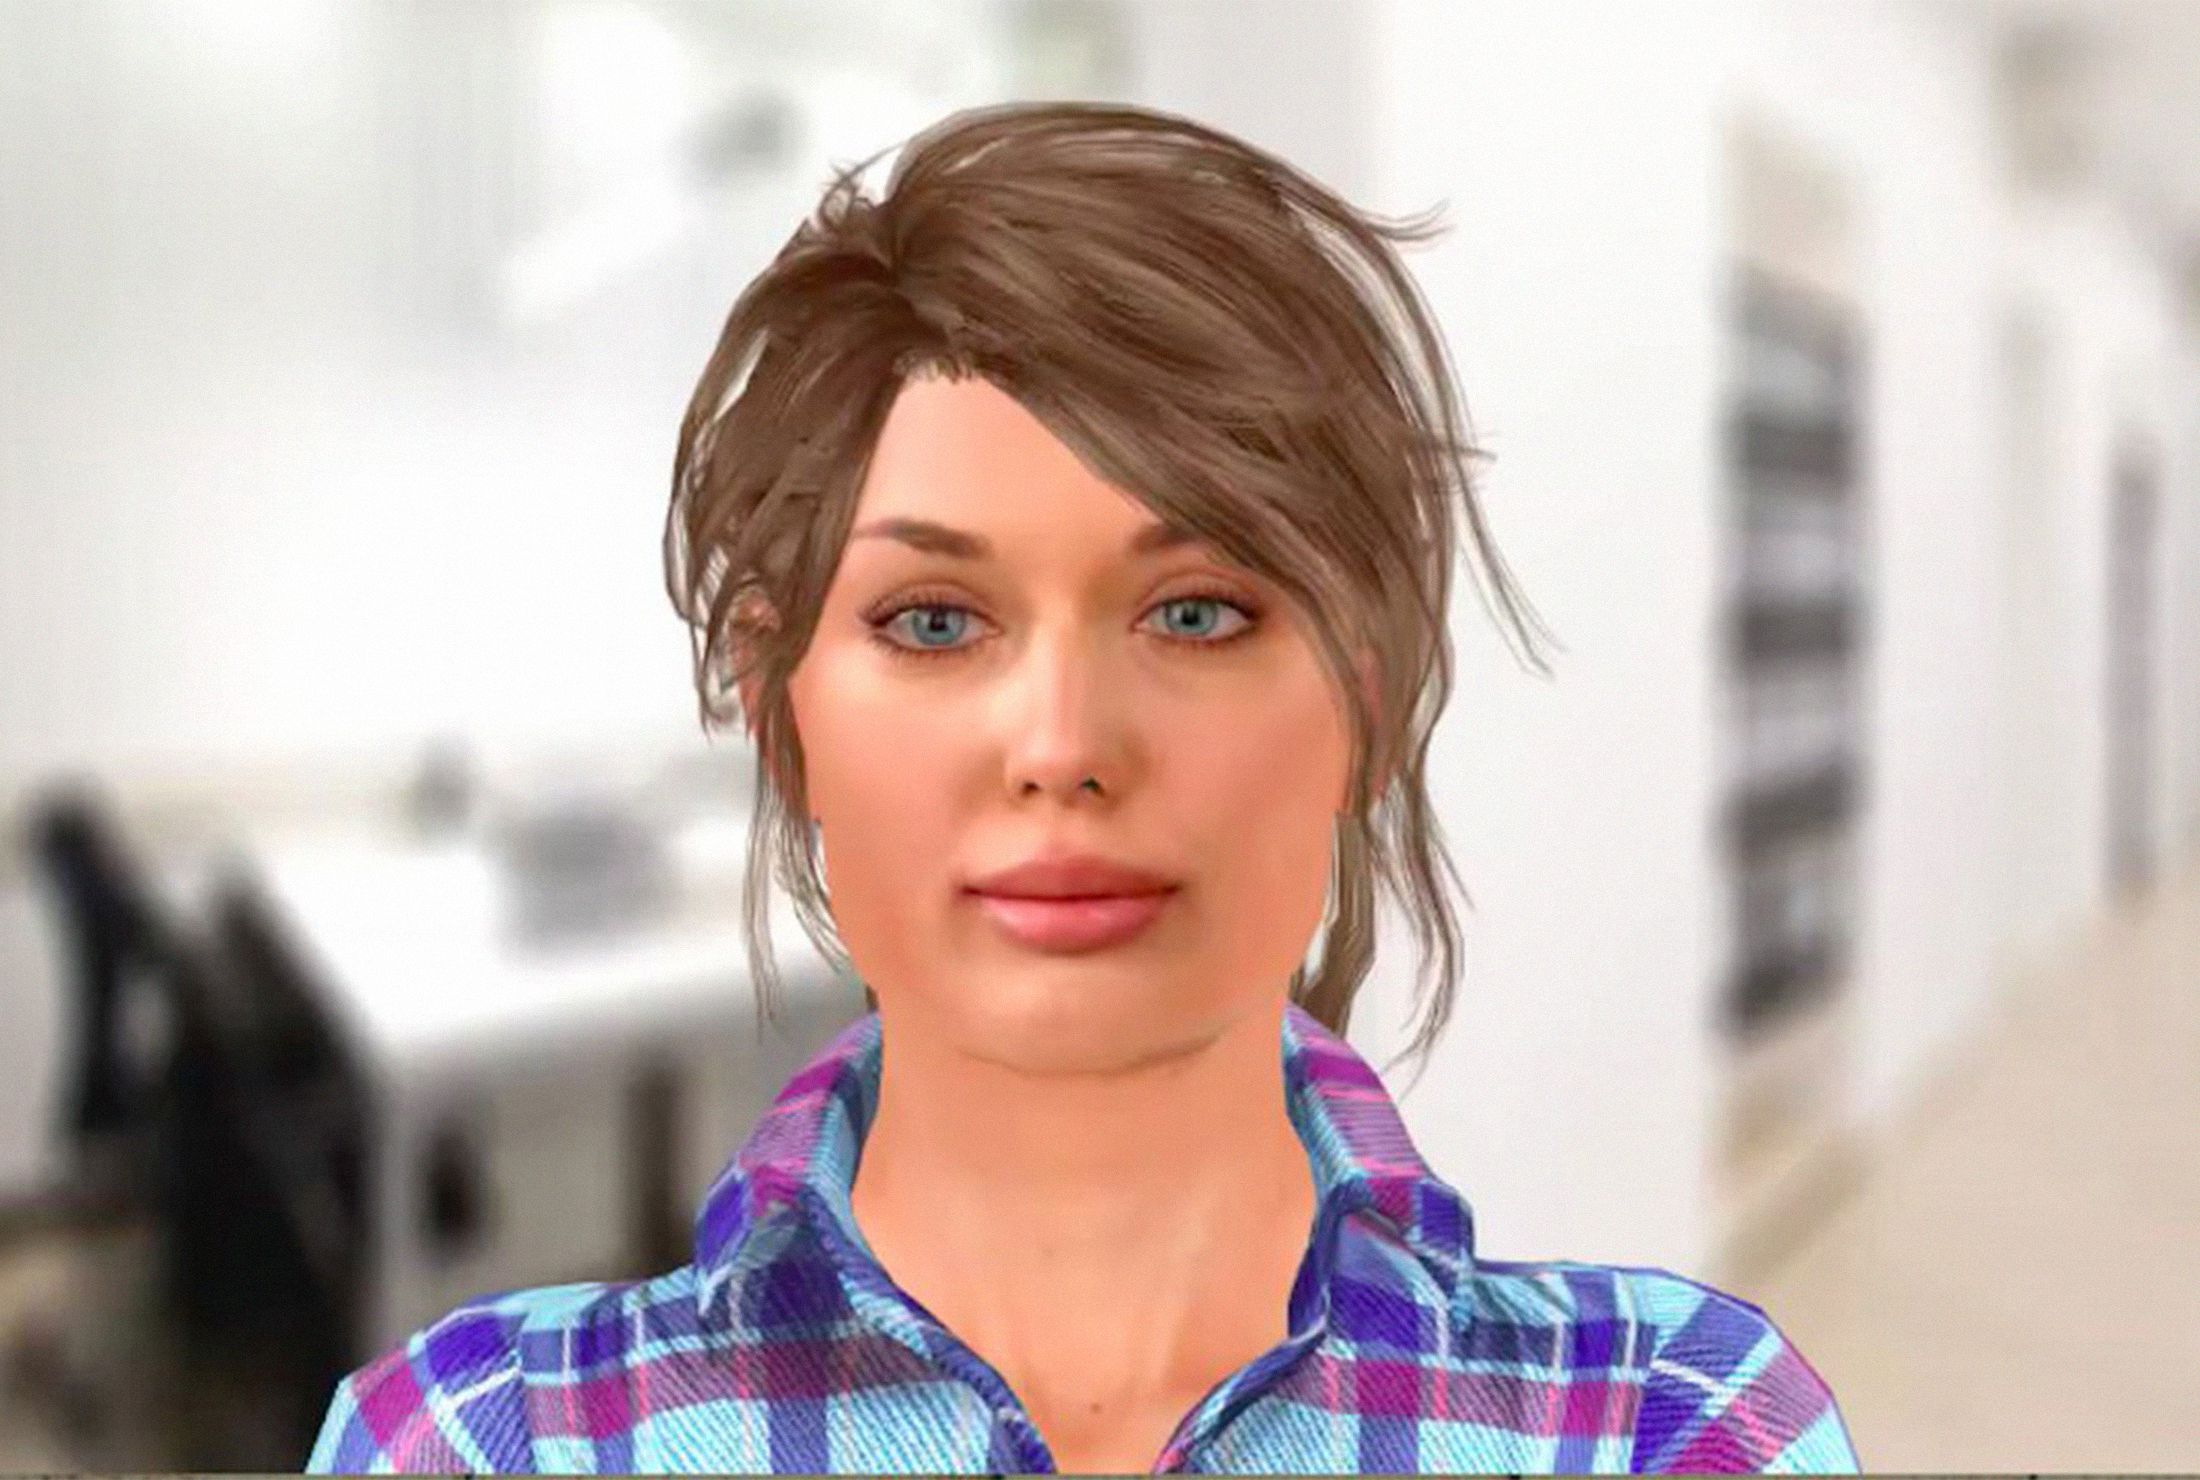
\includegraphics[width=0.26\textwidth]{graphics/study/vera.jpg}}
 \qquad
 \subfloat[\cite{facemaker}\label{fig:image-6}]{%
      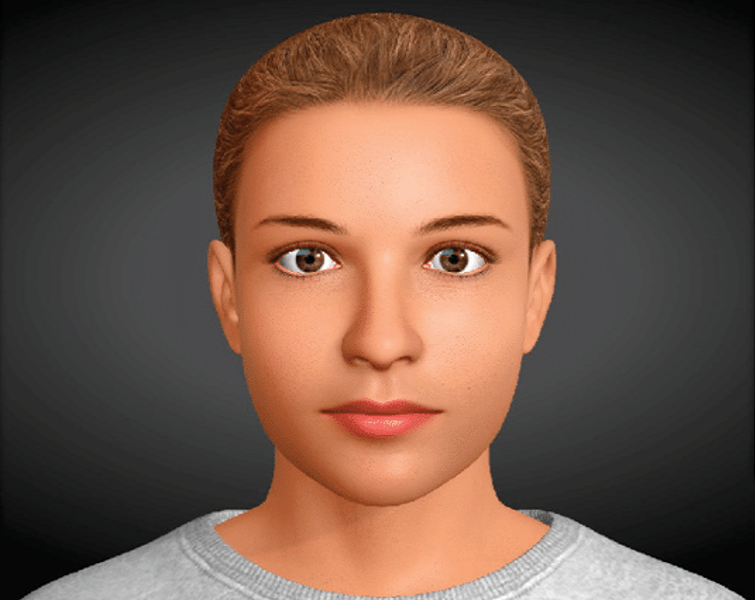
\includegraphics[width=0.26\textwidth]{graphics/study/facemaker.png}}

 \centering
 \subfloat[\cite{knoxfrost}\label{fig:image-7}]{%
      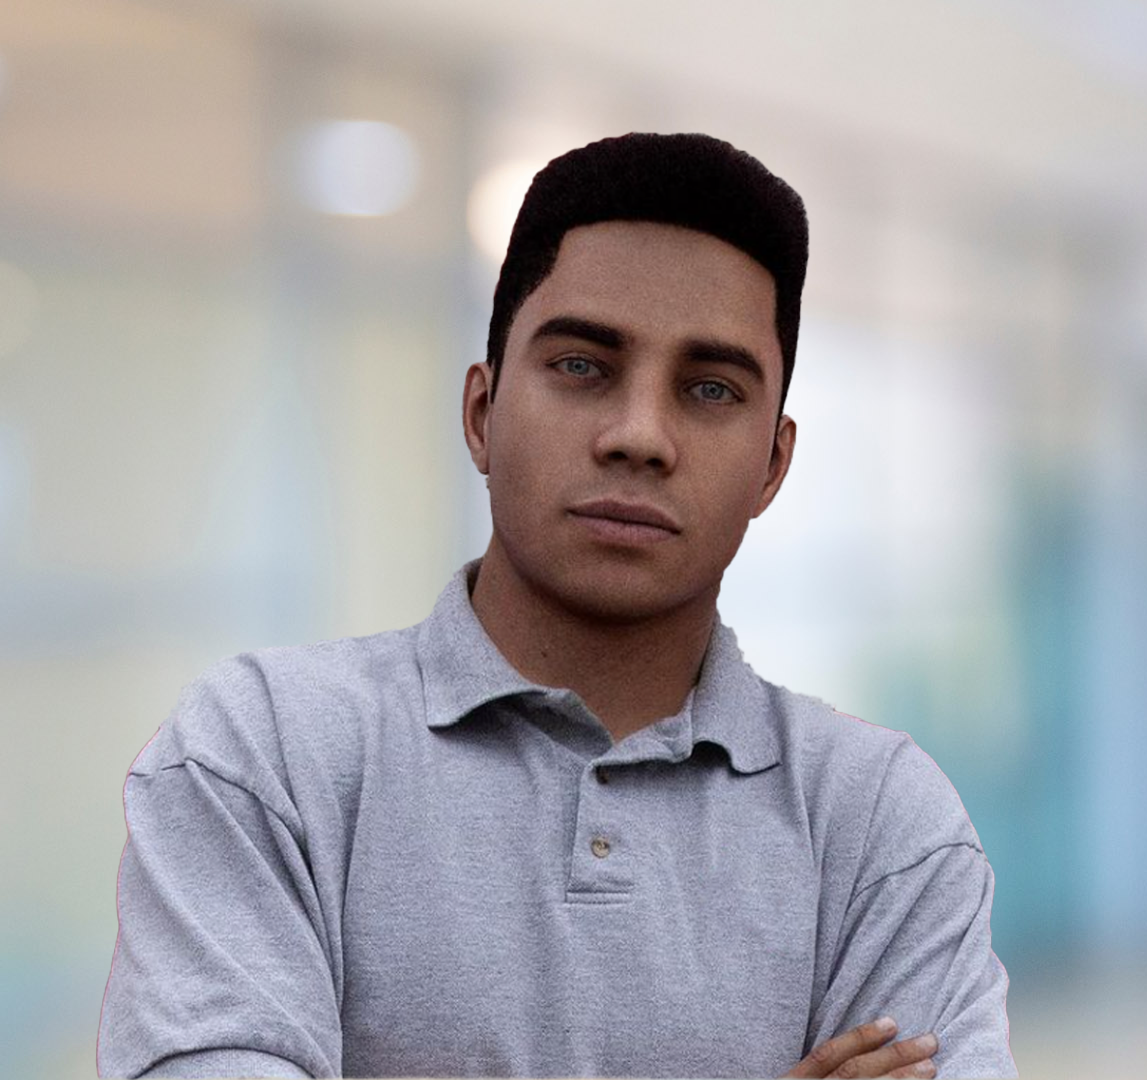
\includegraphics[width=0.26\textwidth]{graphics/study/knoxfrost.png}}
 \qquad
 \subfloat[\cite{emily}\label{fig:image-8}]{%
      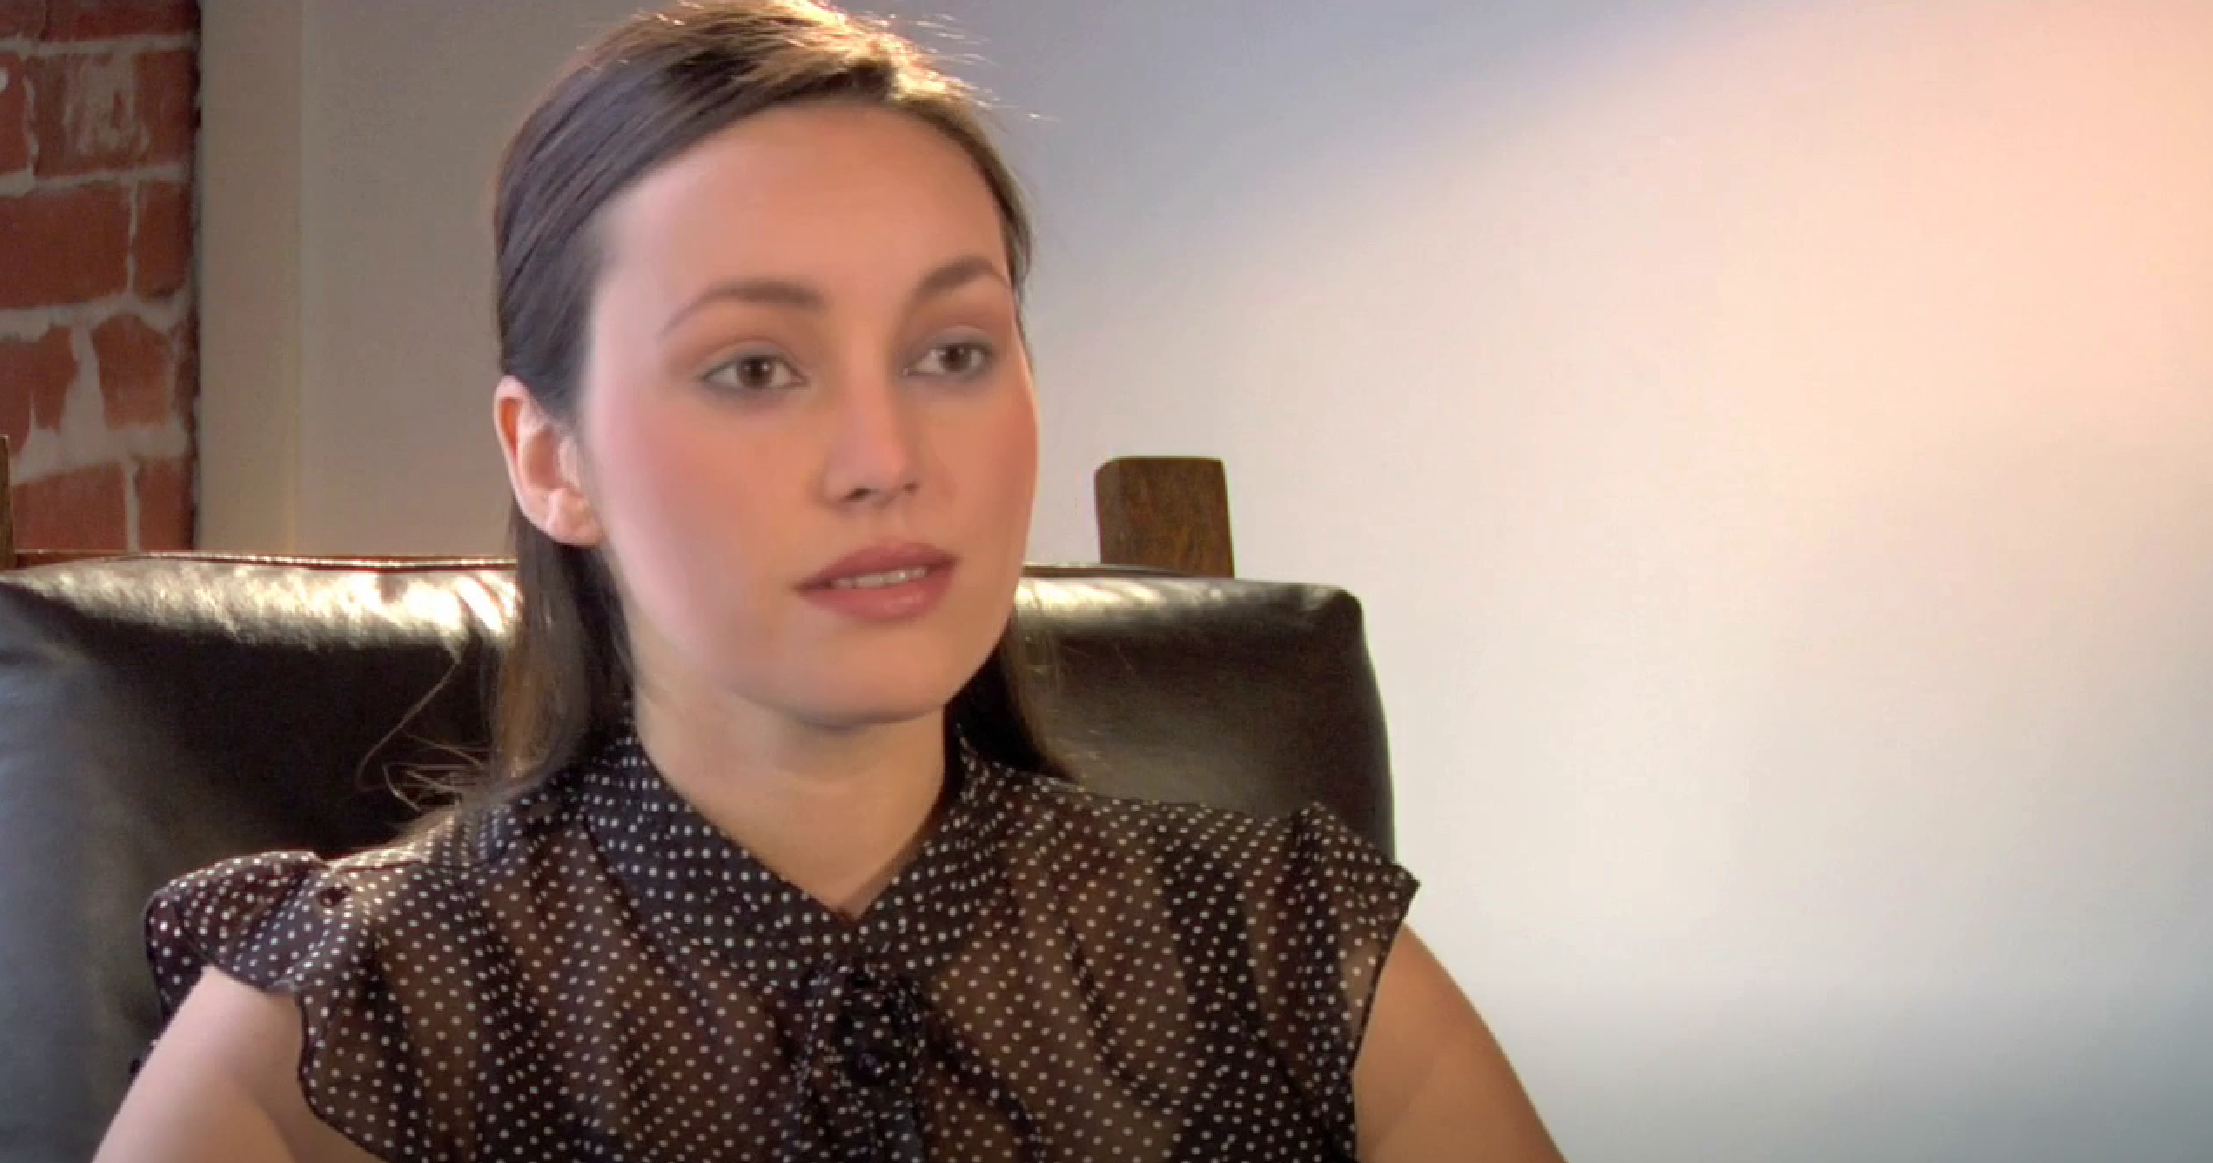
\includegraphics[width=0.26\textwidth]{graphics/study/emily.png}}
 \qquad
 \subfloat[\cite{human}\label{fig:image-9}]{%
      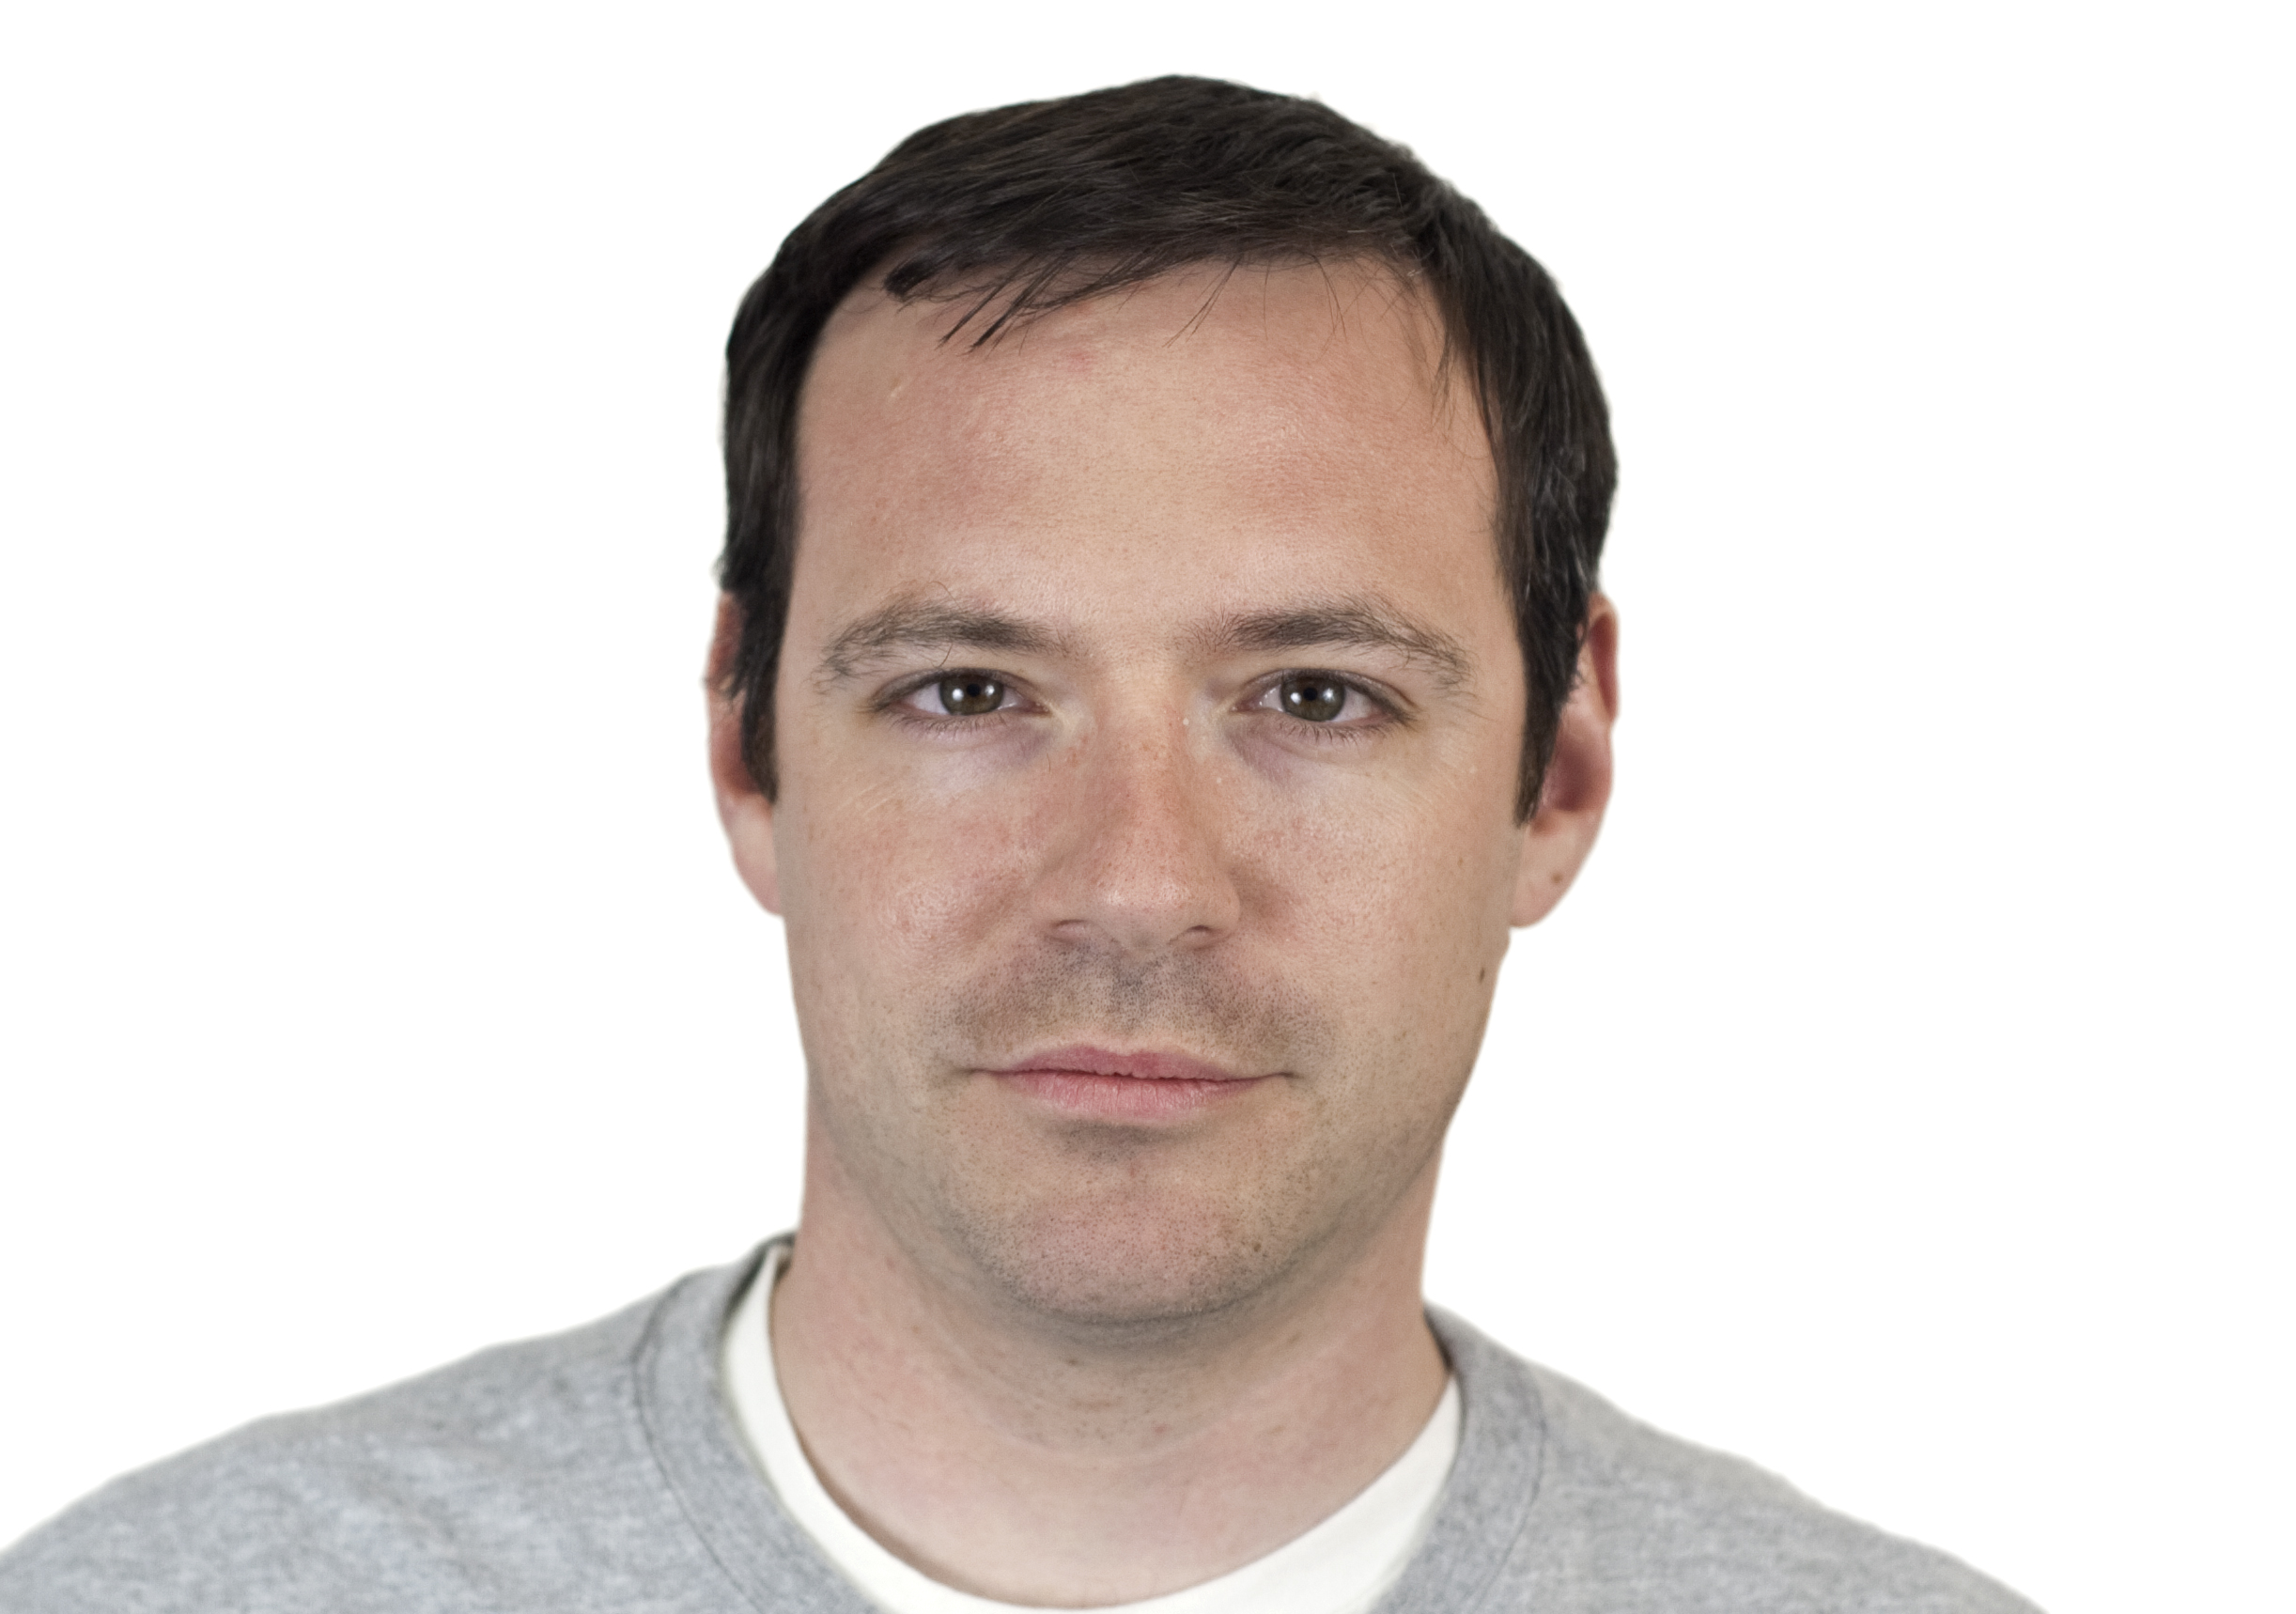
\includegraphics[width=0.26\textwidth]{graphics/study/human.jpg}}
      
\caption{The Entities used in the survey.}
\label{fig:used-entities}

\end{figure}
The focus of the pictures is on the faces of the figures, as this would also be the main focus during a job interview. Furthermore, two of the figures have atypical features. Figure \ref{fig:image-2} depicts a human face with the rest of the body being entirely mechanical, whereas Figure \ref{fig:image-4} depicts a human head with a portion of the skull missing, indicating that it is a robot.

\section{Participants}
A total of 30 people were recruited for the survey. 15 identified as  men, 12 as women, and 3 as non-binary. The age of the participants ranged from 17 to 65 years. The majority of the participants were under the age of 30, with only three over the age of 30 (ages 55 and 65), resulting in a mean age of 26.5. With a total of 27, almost all participants were from Europe, with only three from America.

\section{Method}
This research aims to assess the appearance of various robot recruiters to draw conclusions about their likeability and determine whether they fall into the uncanny valley. To do this, the participants completed a web-based questionnaire in which they had to rate eight images of possible robot recruiters with varying human-likeness and one image of a real human, as seen in Figure 6.1. Before evaluating the robot recruiters, the participants were required to read a brief introductory paragraph. In this text, the following task was described, and the participants were instructed to envision themselves at a job interview employing robot recruiting. Therefore, this introduction should place the chosen entities in the proper context for the rating task. \\
The participants had to rate each of the nine photographs individually in the evaluation assignment. For each picture four 7-point scales between polar adjectives: mechanical/human-like, artificial/lifelike, strange/familiar and not eerie/very eerie were given. In addition, the participants had to indicate how much they liked the picture of the robot recruiter with a simple liking question. Figure \ref{fig:evaluation_task} depicts the exact appearance of the evaluation task questions. The used expressions were also translated into German for better comprehension because most participants were German speakers.
\begin{wrapfigure}[]{r}{0.65\textwidth} %this figure will be at the right
    \centering
    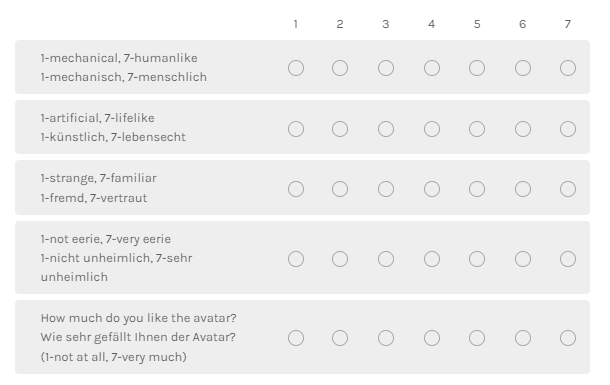
\includegraphics[width=0.65\textwidth]{graphics/evaluation_task.png}
    \caption{Questions used in the evaluation task.}
    \label{fig:evaluation_task}
\end{wrapfigure}
The first two scales (mechanical/human-like, artificial/lifelike)  have the task of inquiring about the perceived human-likeness of the figure for the participant. The other two scales (strange/familiar, not eerie/very eerie) are responsible for evaluating the participants' liking or disliking of the figures. For this thesis I opted to use the still commonly used term `familiar' to describe the sympathy toward the robot recruiters. To give the term `familiar' a greater significance a simple liking question (How much do you like the avatar?) was added to each assessment task of the robot recruiter. This serves to gather more evidence of the connection between familiarity toward a entity and liking an entity.\\
Before beginning the evaluation task, participants were asked to rate how much they notice the usage of computer graphics in new movies and whether they think this is a positive or negative development. Since movies often use computer-generated characters with varying degrees of human-likeness, this question was designed to assess participants' prior experience with virtual characters and the possible prior recognition of the uncanny valley.


\section{Results}
In order to make statements about the different robot recruiter figures, the mean values of the replies from the evaluation task were calculated and illustrated. In the resulting graphs, the x-axis describes the chosen robot recruiter figures, which are ordered in ascending human-likeness as comparable to figure \ref{fig:used-entities}. On the y-axis, the graphs show two or more categories of the 7-point scales, which are set side by side and analysed. The highlighted points in the graphs mark the exact mean values calculated for each figure.\par
\begin{wrapfigure}[]{r}{0.65\textwidth} %this figure will be at the right
    \centering
    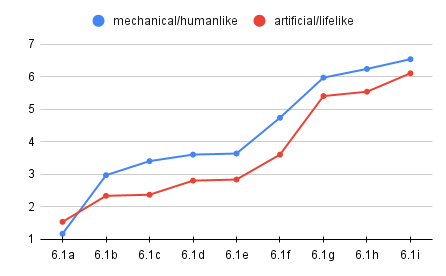
\includegraphics[width=0.65\textwidth]{graphics/result/result1.png}
    \caption{Mean values of the mechanical/humanlike and artificial/lifelike ratings of the avatars.}
    \label{fig:humanlikeness}
    \vspace{20pt}
    \centering
    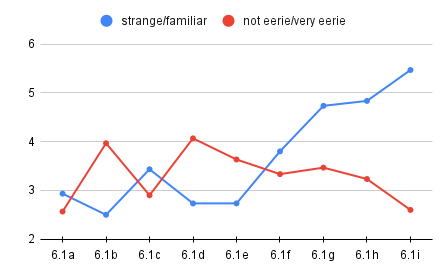
\includegraphics[width=0.65\textwidth]{graphics/result/result2.png}
    \caption{Mean values of the strange/familiar and not eerie/very eerie ratings of the avatars.}
    \label{fig:strangeness}
\end{wrapfigure}
First, the increasing human-likeness of the various entities is evaluated. Graph \ref{fig:humanlikeness} shows the mean scores of the mechanical/humanlike and artificial/lifelike scales for each selected robot recruiter avatar. In this graph, a clear link between human similarity and lifelikeness can be noticed. Furthermore, the human-likeness of the selected avatars clearly increases, as determined by the scores seen in table \ref{tab:rated-human-likeness} from the Abot database human-likeness predictor. The selection of the depicted robot recruiters therefore has been sensibly chosen for an evaluation based on increasing human-likeness.\\
Next, the relationship between the strangeness and eeriness of the characters is considered. From graph \ref{fig:strangeness}, it can be noticed that the more strange a presented robot recruiter was regarded, the more eerie it was likewise rated. Equally, the more familiar a robot recruiter appeared, the less eerie it was rated. As a result, a relation between strangeness and strong eeriness, as well as familiarity and no eeriness, can be observed in the selected figures of this survey. In connection with graph \ref{fig:humanlikeness}, graph \ref{fig:strangeness} already clearly shows how the eeriness of the figures strongly decreases with a very high human resemblance. Whereas the robot recruiters in the midrange of the selected human-likenesses received varying ratings but on average, were rated as more eerie and strange.\par
\begin{wrapfigure}[17]{r}{0.65\textwidth} %this figure will be at the right
    \centering
    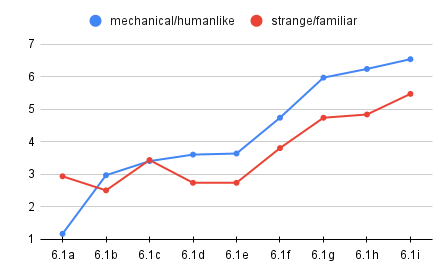
\includegraphics[width=0.65\textwidth]{graphics/result/result3.png}
    \caption{Mean values of the mechanical/humanlike and not strange/familiar ratings of the avatars.}
    \label{fig:uncanny_valley_result}
\end{wrapfigure}
Graph \ref{fig:uncanny_valley_result} shows this relation in more detail, illustrating the mechanical/humanlike and strange/familiar scales for each robot recruiter. The first thing that stands out in this graph is that the mechanical design of figure \ref{fig:image-1}, was assessed with a relatively low level of familiarity. Masahiro Mori's uncanny valley hypothesis predicts that clearly categorisable robots with a moderate human resemblance would be rated with a higher familiarity. The low ranking in this study might, however, be linked to the scenario of a job interview in which the participants should imagine themselves. Since most job interviews are conducted by humans with whom you can interact and who can express emotions, a robot will lose familiarity due to the lack of these characteristics. Familiarity reduces even more with the following figure \ref{fig:image-2}, Tengai, a robot recruiter with both a human and very robot-like design. The loss of familiarity in this entity could arise with the atypical appearance. This robot recruiter combines a completely mechanical body with a very human face. This makes the entire shape of the robot difficult to categorise. This would be further supported by the low rating of figure \ref{fig:image-4}, which also has atypical features and has been rated with little familiarity despite increasing human resemblance. By contrast, figure's \ref{fig:image-3} design shows and increasing familiarity, which can be justified by the increasing human-likeness, its unchallenging categorisation and lack of any atypical features. The next two designs \ref{fig:image-4} and \ref{fig:image-5} are particularly interesting. Here, a drop in familiarity with increasing human-likeness can be observed. Even though only a modest decrease in familiarity can be observed, it is significant and reminiscent of Masahiro Mori's original uncanny valley hypothesis. However, the decrease occurs with less human-likeness than expected, which can be explained by the generally very human-like characters chosen and the absence of movement, interaction or speech. With the following entity, acceptance recovers quickly and rises sharply with the following two selected recruiters. However, no chosen avatar could surpass the human. Even though the robot recruiters' likeability could not surpass that of a human, it appears that the figures \ref{fig:image-7} and \ref{fig:image-8} have escaped the uncanny valley. This could be due to a combination of the figures' nearly perfect human-like appearance and their lack of movement, and the lack of movement which would make the non-human features stand out more.\\
In conclusion, in this study atypical features appear to have contributed to the robot recruiters' uncanny appearance. Additionally the entirely mechanical robot recruiter had an unexpectedly low likeability rating, which could be caused by the lack of familiarity with the use of robots during employment interviews. Finally, although the very human-like designs were able to escape the uncanny valley, no robot recruiter was able to outperform the likeability of the human recruiter.\par
With the last question of the evaluation task, asking the participants how much they liked the robot recruiters to be evaluated, this study wanted to confirm whether the participants associated the chosen term `familiarity' with the affection and liking of the robot recruiters. 
\begin{wrapfigure}[17]{r}{0.65\textwidth} %this figure will be at the right
    \centering
    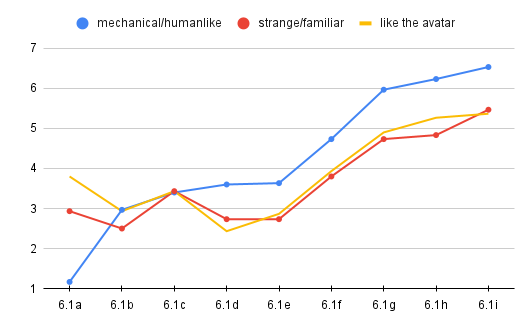
\includegraphics[width=0.65\textwidth]{graphics/result/result4.png}
    \caption{Mean values of the mechanical/humanlike, strange/familiar and liking ratings of the avatars.}
    \label{fig:likeability}
\end{wrapfigure}
Therefore, graph \ref{fig:likeability} compares the mean values of the strange/familiar and the simple liking questions ratings. In addition, the graph shows the human-likeness of the avatars to illustrate their order clearly. Undoubtedly in this survey, the liking question's ratings are nearly identical to the ratings between strange and familiar. Only in the case of a purely mechanical design, the character's liking is slightly greater than the familiarity rating. Overall, the ratings between strange and familiar and the liking question are almost alike, which means that in this study a clear link can be established between the liking of an robot recruiter and its familiarity.\\
In order to better assess the participants' previous experience and personal susceptibility to the uncanny valley, two questions on the use of computer-generated graphics in films had to be answered before the robot recruiters were evaluated. Films are one of the mediums through which many people are exposed to the uncanny valley. The first question asked participants how much they noticed the use of computer graphics on a scale from 1 (very little) to 7 (very much) in films. With a mean score of 5.6, the participants in this survey noticed the use of computer graphics strongly, which speaks for a very attentive group of people with regard to the usage of virtual graphics and thus also the uncanny valley effect. The second question asked the participants whether they noticed the use of such in a positive or negative way on a scale of 1 (very negative) to 7 (very positive). With a mean score of 5.4, the participants in this study notice the use of computer graphics as a positive development. From these questions, this study theorises that most participants have already been exposed to the uncanny valley in some form in films. However, since most participants perceive the use of effects positively, it could be argued that virtual characters in films that fall into the uncanny valley are also more likely to be perceived positively by the participants. This could have had an effect on better ratings of the almost human-like robot recruiters.

\section{Discussion}
In this study, the degree of anthropomorphism of the robot recruiters had a substantial impact on their likeability. Furthermore, an uncanny valley can be recognised in the highly human-like but not entirely human-like figures \ref{fig:image-4} and \ref{fig:image-5}. However, the uncanny valley effect observed in this study is weaker than predicted in the original hypothesis by Masahiro Mori. One of the main reasons for this might be the robot recruiters' lack of movement, interaction, and voices. Moreover, contrary to Masahiro Mori's hypothesis, the completely mechanical robot recruiter was rated less likeable than expected. This could be attributable to the fact that the participants were asked to imagine the robot recruiters during a job interview. As robots are not common in employment interviews yet, this may have caused additional rejection in the participants.
Interestingly, the almost perfectly human-like robot recruiters were able to escape the uncanny valley even though they were not rated better than humans. In addition to the near-flawless human resemblance, this could also be due to the lack of movement and interaction with the robot recruiters, which would have emphasised their imperfections. 
Overall, the robot recruiters in this study with a high degree of human-likeness seem to be  associated with an increase in their likeability. Robot recruiters with a high degree of human-likeness but plainly abnormal design elements or atypical bodies, such as a combination of a mechanical and human appearance, have a low likeability and have fallen into the uncanny valley.
The mechanical robot recruiter was also rated poorly by the participants, which further speaks for the importance of a human design for robot recruiters.\\
This study was confined to a relatively small number of participants and a selected number of possible static images of robot recruiters. Furthermore, the participants' average age was quite young, and they all came from a western ethnic background. To confirm the results of this study and to increase the research on the uncanny valley in robot recruiters, the study should be repeated with a larger number of participants from diverse cultures and different age groups.
Furthermore, the integration of movement, language and possibly the direct interaction with the robot recruiters would be significant factors that could lead to different evaluations of their likeability. With the likely increase in the use of robot recruiters in the coming years, further research into the interaction between robot recruiters and the impact of their appearance on their acceptance and likeability is needed. 

\backmatter

\listoffigures % Starred version, i.e., \listoffigures*, removes the toc entry.

% Use an optional list of tables.
%\cleardoublepage % Start list of tables on the next empty right hand page.
%\listoftables % Starred version, i.e., \listoftables*, removes the toc entry.

% Use an optional list of alogrithms.
%\listofalgorithms
%\addcontentsline{toc}{chapter}{List of Algorithms}

% Add an index.
%\printindex

% Add a glossary.
%\printglossaries

% Add a bibliography.
\bibliographystyle{apalike}
\bibliography{refs}

\end{document}